% !mode::"TeX:UTF-8"
%!TEX program = xelatex
% +-----------------------------------------------------------------------------
% | File: seminar notes
% | Author: Zhang Hao
% |
% | 
% | 
% | Description:
% |     一些笔记和讲义
% |
% | 
% | 
% +-----------------------------------------------------------------------------
% !mode::"TeX:UTF-8"
% !TEX program = xelatex
% +-----------------------------------------------------------------------------
% | File: 格式文档
% | 
% |
% | 
% | 
% | Description:
% |   主要是为了方便而设立。  
% |   使用% !mode::"TeX:UTF-8"
% !TEX program = xelatex
% +-----------------------------------------------------------------------------
% | File: 格式文档
% | 
% |
% | 
% | 
% | Description:
% |   主要是为了方便而设立。  
% |   使用% !mode::"TeX:UTF-8"
% !TEX program = xelatex
% +-----------------------------------------------------------------------------
% | File: 格式文档
% | 
% |
% | 
% | 
% | Description:
% |   主要是为了方便而设立。  
% |   使用\include{format} 加载本文档
% | 
% | 
% +-----------------------------------------------------------------------------
\documentclass[openany,leqno,11pt]{book}  %ctexart,article

\usepackage{imakeidx}
\usepackage{multicol,multirow} % used for the two-column index 多行多列, 在表格中会用到
\usepackage[bottom]{footmisc}
\usepackage{url}  %这个是加超链接
\usepackage{indentfirst} %首行缩进
\usepackage{bm,amscd,xy,amssymb,amsmath,amsthm,nicefrac,amsfonts,pifont,mathtools,xltxtra}
\usepackage{ctex}
\usepackage{colortbl}
\usepackage{graphicx}
\usepackage{longtable}
\usepackage{booktabs}
% \usepackage{calrsfs} %代数几何中mathcal字体转换 
\usepackage{stmaryrd}% 打\mapsfrom 还有幂级数的符号 \llbracket \rrbracket
% \usepackage{alggp} %代数群文档专用,其中有一些命令由于冲突注销了,如果单独使用,请取消注销

\usepackage{cite} %引用参考文献

%----和后文制作封面一起使用的,如果不通过编译,还是置于后面
%----据说是要放在tikz宏包前面
\usepackage[svgnames]{xcolor} % Required to specify font color

% \newcommand*{\plogo}{\fbox{$\mathcal{PL}$}} % Generic publisher logo %logo 没啥意思

\usepackage{graphicx} % Required for box manipulation
%----
\usepackage{tikz}
	% \usetikzlibrary{cd}
\usepackage{tikz-cd} %xymatrix包文中用过几处, 后来都是在用tikz-cd来画交换图
\xyoption{all}
\newdir{ >}{{}*!/-5pt/@{>}}
% \usepackage{microtype} %microtype 宏包可以改善了单词、字母的间距。它可能做了很多, 但是大部分人察觉不到使用它之后文档的变化。但至少, 加载了 microtype 之后, 文档看起来更好, 也更容易阅读。注意:如果有使用到字体宏包, 需要将 microtype 宏包放在它们的后面, 因为这个宏包对单词、字母的调整和字体是有关的。

\usepackage[pdfencoding=auto,psdextra]{hyperref} % hyperref还是有些小问题,比如section的名字里不能有数学符号,需要用特殊的命令处理掉它。
\usepackage{bookmark}
\renewcommand\bibname{参考文献} %修改bib的名称

%improving spacing in tables (space above and below characters in a row)
\newcommand{\tfix}{\rule{0pt}{2.6ex}}
\newcommand{\bfix}{\rule[-1.2ex]{0pt}{0pt}}

%--一些数学符号, 常用的有\Hom \End \iso(向右箭头上有同构) \id \ker \ima \coker \tor \ext \N \Z \Q \R \mathbb{C}
\newcommand{\Hom}{\mathop{\mathrm{Hom}}} %这个常用
\newcommand{\End}{\mathrm{End}}
\newcommand{\Nil}{\mathrm{Nil}}
\newcommand{\rank}{\mathrm{rank\ }}
\newcommand{\ord}{\mathrm{ord}}
\newcommand{\tr}{\mathrm{tr}}
\newcommand{\id}{\mathrm{id}} %这个常用
\newcommand{\coker}{\mathrm{coker}}
%\newcommand{\ker}{\mathrm{ker}} %\ker直接输入就好
\newcommand{\tor}{\mathrm{Tor}}
\newcommand{\ext}{\mathrm{Ext}}
\newcommand{\ima}{\mathrm{Im}}
\newcommand{\N}{\mathbb{N}}
\newcommand{\Z}{\mathbb{Z}}
\newcommand{\Zn}[1]{\Z/{#1}\Z}
\newcommand{\Q}{\mathbb{Q}}
\newcommand{\R}{\mathbb{R}}
% \newcommand{\C}{\mathbb{C}}  %注销这个的原因是\C 和hyperref宏包冲突。后放弃hyperref,还是有很多冲突,比如页码不对
\newcommand{\F}{\mathbb{F}}

%范畴学常用
\newcommand{\J}{\mathcal{J}}  
\newcommand{\cC}{\mathcal{C}} 
\newcommand{\Top}{\mathbf{Top}}
\newcommand{\Ab}{\mathbf{Ab}}
\newcommand{\Grp}{\mathbf{Grp}}
\newcommand{\Obj}{\mathop{\mathrm{Obj}}}
\newcommand{\sets}{\mathrm{Sets}}
\newcommand*{\colim}{\mathop{\mathrm{colim}}}
\newcommand{\coeq}{\mathrm{coeq}}
\newcommand{\coli}{\colim}

%一些箭头
\newcommand{\iso}{\overset{\cong}{\to}} %isomorphic 这个\to 可以换成\longrightarrow 变长
\newcommand{\weq}{\overset{\sim}{\to}} %表示weak equivalence
\newcommand{\cofi}{\rightarrowtail} %带尾巴的箭头, 单射或者余纤维cofibration
\newcommand{\fib}{\twoheadrightarrow} %满射 或者纤维化fibration
\newcommand{\defo}{\overset{\sim}{\fib}} %这个没用过
\newcommand{\DA}{\Delta} %一般也不用

\def\idem{\mathrm{Idem}}
\renewcommand{\inf}{\rm inf}
\newcommand{\nil}{\rm nil}
\newcommand{\ass}{\mathrm{Ass}}
\newcommand{\der}{\mathrm{Der}}

%Here are some user-defined operators
\newcommand{\Tr}{\operatorname {Tr}}
\newcommand{\GL}{\operatorname {GL}}
\newcommand{\SL}{\operatorname {SL}}

%------这个部分包含了计数器,使得定理,引理等按照同一顺序编号
\newtheorem{theorem}{Theorem}[chapter]
\renewcommand\thetheorem{\arabic{chapter}.\arabic{theorem}} 
\newtheorem{lemma}[theorem]{Lemma}
\renewcommand\thelemma{\arabic{chapter}.\arabic{lemma}} 
\newtheorem{prop}[theorem]{Proposition}
\renewcommand\theprop{\arabic{chapter}.\arabic{prop}} 
\newtheorem{corollary}[theorem]{Corollary}
\renewcommand\thecorollary{\arabic{chapter}.\arabic{corollary}} 
\renewcommand\theequation{\thetheorem}
\newtheorem{conjecture}[theorem]{Conjecture}
\newtheorem*{theorem*}{Theorem}
\newtheorem*{corollary*}{Corollary}
\newtheorem*{lemma*}{Lemma}

%These deal with definition-like environments (i.e., non-italic)
\theoremstyle{definition}
\newtheorem{definition}[theorem]{Definition}
\newtheorem{example}[theorem]{Example}
\newtheorem{remark}[theorem]{Remark}
\newtheorem*{definition*}{Definition}
\newtheorem*{example*}{Example}
\newtheorem*{remark*}{Remark}
\renewcommand\theexample{\arabic{chapter}.\arabic{example}} 

\makeindex
\setlength{\textwidth}{16cm} \setlength{\textheight}{22cm}
\setlength{\oddsidemargin}{0.5cm} \setlength{\topmargin}{0cm}
\setlength{\evensidemargin}{0.5cm} \setlength{\topmargin}{0cm}
% \usepackage[text={150mm,195mm},centering]{geometry}
% \usepackage[body={16cm,24cm}, top=3cm]{geometry}
% 修改列表环境下行间距 2016.3.11
\usepackage{paralist}
\let\itemize\compactitem
\let\enditemize\endcompactitem
\let\enumerate\compactenum
\let\endenumerate\endcompactenum
\let\description\compactdesc
\let\enddescription\endcompactdesc

% \setlength{\pltopsep}{7pt}
% \setlength{\pltopsep}{10pt}

%修改英文字体  这个字体挺好看的 下面两句都是重要的
\usepackage[T1]{fontenc} % The default font encoding only contains Latin characters
\usepackage[noBBpl]{mathpazo} 加载本文档
% | 
% | 
% +-----------------------------------------------------------------------------
\documentclass[openany,leqno,11pt]{book}  %ctexart,article

\usepackage{imakeidx}
\usepackage{multicol,multirow} % used for the two-column index 多行多列, 在表格中会用到
\usepackage[bottom]{footmisc}
\usepackage{url}  %这个是加超链接
\usepackage{indentfirst} %首行缩进
\usepackage{bm,amscd,xy,amssymb,amsmath,amsthm,nicefrac,amsfonts,pifont,mathtools,xltxtra}
\usepackage{ctex}
\usepackage{colortbl}
\usepackage{graphicx}
\usepackage{longtable}
\usepackage{booktabs}
% \usepackage{calrsfs} %代数几何中mathcal字体转换 
\usepackage{stmaryrd}% 打\mapsfrom 还有幂级数的符号 \llbracket \rrbracket
% \usepackage{alggp} %代数群文档专用,其中有一些命令由于冲突注销了,如果单独使用,请取消注销

\usepackage{cite} %引用参考文献

%----和后文制作封面一起使用的,如果不通过编译,还是置于后面
%----据说是要放在tikz宏包前面
\usepackage[svgnames]{xcolor} % Required to specify font color

% \newcommand*{\plogo}{\fbox{$\mathcal{PL}$}} % Generic publisher logo %logo 没啥意思

\usepackage{graphicx} % Required for box manipulation
%----
\usepackage{tikz}
	% \usetikzlibrary{cd}
\usepackage{tikz-cd} %xymatrix包文中用过几处, 后来都是在用tikz-cd来画交换图
\xyoption{all}
\newdir{ >}{{}*!/-5pt/@{>}}
% \usepackage{microtype} %microtype 宏包可以改善了单词、字母的间距。它可能做了很多, 但是大部分人察觉不到使用它之后文档的变化。但至少, 加载了 microtype 之后, 文档看起来更好, 也更容易阅读。注意:如果有使用到字体宏包, 需要将 microtype 宏包放在它们的后面, 因为这个宏包对单词、字母的调整和字体是有关的。

\usepackage[pdfencoding=auto,psdextra]{hyperref} % hyperref还是有些小问题,比如section的名字里不能有数学符号,需要用特殊的命令处理掉它。
\usepackage{bookmark}
\renewcommand\bibname{参考文献} %修改bib的名称

%improving spacing in tables (space above and below characters in a row)
\newcommand{\tfix}{\rule{0pt}{2.6ex}}
\newcommand{\bfix}{\rule[-1.2ex]{0pt}{0pt}}

%--一些数学符号, 常用的有\Hom \End \iso(向右箭头上有同构) \id \ker \ima \coker \tor \ext \N \Z \Q \R \mathbb{C}
\newcommand{\Hom}{\mathop{\mathrm{Hom}}} %这个常用
\newcommand{\End}{\mathrm{End}}
\newcommand{\Nil}{\mathrm{Nil}}
\newcommand{\rank}{\mathrm{rank\ }}
\newcommand{\ord}{\mathrm{ord}}
\newcommand{\tr}{\mathrm{tr}}
\newcommand{\id}{\mathrm{id}} %这个常用
\newcommand{\coker}{\mathrm{coker}}
%\newcommand{\ker}{\mathrm{ker}} %\ker直接输入就好
\newcommand{\tor}{\mathrm{Tor}}
\newcommand{\ext}{\mathrm{Ext}}
\newcommand{\ima}{\mathrm{Im}}
\newcommand{\N}{\mathbb{N}}
\newcommand{\Z}{\mathbb{Z}}
\newcommand{\Zn}[1]{\Z/{#1}\Z}
\newcommand{\Q}{\mathbb{Q}}
\newcommand{\R}{\mathbb{R}}
% \newcommand{\C}{\mathbb{C}}  %注销这个的原因是\C 和hyperref宏包冲突。后放弃hyperref,还是有很多冲突,比如页码不对
\newcommand{\F}{\mathbb{F}}

%范畴学常用
\newcommand{\J}{\mathcal{J}}  
\newcommand{\cC}{\mathcal{C}} 
\newcommand{\Top}{\mathbf{Top}}
\newcommand{\Ab}{\mathbf{Ab}}
\newcommand{\Grp}{\mathbf{Grp}}
\newcommand{\Obj}{\mathop{\mathrm{Obj}}}
\newcommand{\sets}{\mathrm{Sets}}
\newcommand*{\colim}{\mathop{\mathrm{colim}}}
\newcommand{\coeq}{\mathrm{coeq}}
\newcommand{\coli}{\colim}

%一些箭头
\newcommand{\iso}{\overset{\cong}{\to}} %isomorphic 这个\to 可以换成\longrightarrow 变长
\newcommand{\weq}{\overset{\sim}{\to}} %表示weak equivalence
\newcommand{\cofi}{\rightarrowtail} %带尾巴的箭头, 单射或者余纤维cofibration
\newcommand{\fib}{\twoheadrightarrow} %满射 或者纤维化fibration
\newcommand{\defo}{\overset{\sim}{\fib}} %这个没用过
\newcommand{\DA}{\Delta} %一般也不用

\def\idem{\mathrm{Idem}}
\renewcommand{\inf}{\rm inf}
\newcommand{\nil}{\rm nil}
\newcommand{\ass}{\mathrm{Ass}}
\newcommand{\der}{\mathrm{Der}}

%Here are some user-defined operators
\newcommand{\Tr}{\operatorname {Tr}}
\newcommand{\GL}{\operatorname {GL}}
\newcommand{\SL}{\operatorname {SL}}

%------这个部分包含了计数器,使得定理,引理等按照同一顺序编号
\newtheorem{theorem}{Theorem}[chapter]
\renewcommand\thetheorem{\arabic{chapter}.\arabic{theorem}} 
\newtheorem{lemma}[theorem]{Lemma}
\renewcommand\thelemma{\arabic{chapter}.\arabic{lemma}} 
\newtheorem{prop}[theorem]{Proposition}
\renewcommand\theprop{\arabic{chapter}.\arabic{prop}} 
\newtheorem{corollary}[theorem]{Corollary}
\renewcommand\thecorollary{\arabic{chapter}.\arabic{corollary}} 
\renewcommand\theequation{\thetheorem}
\newtheorem{conjecture}[theorem]{Conjecture}
\newtheorem*{theorem*}{Theorem}
\newtheorem*{corollary*}{Corollary}
\newtheorem*{lemma*}{Lemma}

%These deal with definition-like environments (i.e., non-italic)
\theoremstyle{definition}
\newtheorem{definition}[theorem]{Definition}
\newtheorem{example}[theorem]{Example}
\newtheorem{remark}[theorem]{Remark}
\newtheorem*{definition*}{Definition}
\newtheorem*{example*}{Example}
\newtheorem*{remark*}{Remark}
\renewcommand\theexample{\arabic{chapter}.\arabic{example}} 

\makeindex
\setlength{\textwidth}{16cm} \setlength{\textheight}{22cm}
\setlength{\oddsidemargin}{0.5cm} \setlength{\topmargin}{0cm}
\setlength{\evensidemargin}{0.5cm} \setlength{\topmargin}{0cm}
% \usepackage[text={150mm,195mm},centering]{geometry}
% \usepackage[body={16cm,24cm}, top=3cm]{geometry}
% 修改列表环境下行间距 2016.3.11
\usepackage{paralist}
\let\itemize\compactitem
\let\enditemize\endcompactitem
\let\enumerate\compactenum
\let\endenumerate\endcompactenum
\let\description\compactdesc
\let\enddescription\endcompactdesc

% \setlength{\pltopsep}{7pt}
% \setlength{\pltopsep}{10pt}

%修改英文字体  这个字体挺好看的 下面两句都是重要的
\usepackage[T1]{fontenc} % The default font encoding only contains Latin characters
\usepackage[noBBpl]{mathpazo} 加载本文档
% | 
% | 
% +-----------------------------------------------------------------------------
\documentclass[openany,leqno,11pt]{book}  %ctexart,article

\usepackage{imakeidx}
\usepackage{multicol,multirow} % used for the two-column index 多行多列, 在表格中会用到
\usepackage[bottom]{footmisc}
\usepackage{url}  %这个是加超链接
\usepackage{indentfirst} %首行缩进
\usepackage{bm,amscd,xy,amssymb,amsmath,amsthm,nicefrac,amsfonts,pifont,mathtools,xltxtra}
\usepackage{ctex}
\usepackage{colortbl}
\usepackage{graphicx}
\usepackage{longtable}
\usepackage{booktabs}
% \usepackage{calrsfs} %代数几何中mathcal字体转换 
\usepackage{stmaryrd}% 打\mapsfrom 还有幂级数的符号 \llbracket \rrbracket
% \usepackage{alggp} %代数群文档专用,其中有一些命令由于冲突注销了,如果单独使用,请取消注销

\usepackage{cite} %引用参考文献

%----和后文制作封面一起使用的,如果不通过编译,还是置于后面
%----据说是要放在tikz宏包前面
\usepackage[svgnames]{xcolor} % Required to specify font color

% \newcommand*{\plogo}{\fbox{$\mathcal{PL}$}} % Generic publisher logo %logo 没啥意思

\usepackage{graphicx} % Required for box manipulation
%----
\usepackage{tikz}
	% \usetikzlibrary{cd}
\usepackage{tikz-cd} %xymatrix包文中用过几处, 后来都是在用tikz-cd来画交换图
\xyoption{all}
\newdir{ >}{{}*!/-5pt/@{>}}
% \usepackage{microtype} %microtype 宏包可以改善了单词、字母的间距。它可能做了很多, 但是大部分人察觉不到使用它之后文档的变化。但至少, 加载了 microtype 之后, 文档看起来更好, 也更容易阅读。注意:如果有使用到字体宏包, 需要将 microtype 宏包放在它们的后面, 因为这个宏包对单词、字母的调整和字体是有关的。

\usepackage[pdfencoding=auto,psdextra]{hyperref} % hyperref还是有些小问题,比如section的名字里不能有数学符号,需要用特殊的命令处理掉它。
\usepackage{bookmark}
\renewcommand\bibname{参考文献} %修改bib的名称

%improving spacing in tables (space above and below characters in a row)
\newcommand{\tfix}{\rule{0pt}{2.6ex}}
\newcommand{\bfix}{\rule[-1.2ex]{0pt}{0pt}}

%--一些数学符号, 常用的有\Hom \End \iso(向右箭头上有同构) \id \ker \ima \coker \tor \ext \N \Z \Q \R \mathbb{C}
\newcommand{\Hom}{\mathop{\mathrm{Hom}}} %这个常用
\newcommand{\End}{\mathrm{End}}
\newcommand{\Nil}{\mathrm{Nil}}
\newcommand{\rank}{\mathrm{rank\ }}
\newcommand{\ord}{\mathrm{ord}}
\newcommand{\tr}{\mathrm{tr}}
\newcommand{\id}{\mathrm{id}} %这个常用
\newcommand{\coker}{\mathrm{coker}}
%\newcommand{\ker}{\mathrm{ker}} %\ker直接输入就好
\newcommand{\tor}{\mathrm{Tor}}
\newcommand{\ext}{\mathrm{Ext}}
\newcommand{\ima}{\mathrm{Im}}
\newcommand{\N}{\mathbb{N}}
\newcommand{\Z}{\mathbb{Z}}
\newcommand{\Zn}[1]{\Z/{#1}\Z}
\newcommand{\Q}{\mathbb{Q}}
\newcommand{\R}{\mathbb{R}}
% \newcommand{\C}{\mathbb{C}}  %注销这个的原因是\C 和hyperref宏包冲突。后放弃hyperref,还是有很多冲突,比如页码不对
\newcommand{\F}{\mathbb{F}}

%范畴学常用
\newcommand{\J}{\mathcal{J}}  
\newcommand{\cC}{\mathcal{C}} 
\newcommand{\Top}{\mathbf{Top}}
\newcommand{\Ab}{\mathbf{Ab}}
\newcommand{\Grp}{\mathbf{Grp}}
\newcommand{\Obj}{\mathop{\mathrm{Obj}}}
\newcommand{\sets}{\mathrm{Sets}}
\newcommand*{\colim}{\mathop{\mathrm{colim}}}
\newcommand{\coeq}{\mathrm{coeq}}
\newcommand{\coli}{\colim}

%一些箭头
\newcommand{\iso}{\overset{\cong}{\to}} %isomorphic 这个\to 可以换成\longrightarrow 变长
\newcommand{\weq}{\overset{\sim}{\to}} %表示weak equivalence
\newcommand{\cofi}{\rightarrowtail} %带尾巴的箭头, 单射或者余纤维cofibration
\newcommand{\fib}{\twoheadrightarrow} %满射 或者纤维化fibration
\newcommand{\defo}{\overset{\sim}{\fib}} %这个没用过
\newcommand{\DA}{\Delta} %一般也不用

\def\idem{\mathrm{Idem}}
\renewcommand{\inf}{\rm inf}
\newcommand{\nil}{\rm nil}
\newcommand{\ass}{\mathrm{Ass}}
\newcommand{\der}{\mathrm{Der}}

%Here are some user-defined operators
\newcommand{\Tr}{\operatorname {Tr}}
\newcommand{\GL}{\operatorname {GL}}
\newcommand{\SL}{\operatorname {SL}}

%------这个部分包含了计数器,使得定理,引理等按照同一顺序编号
\newtheorem{theorem}{Theorem}[chapter]
\renewcommand\thetheorem{\arabic{chapter}.\arabic{theorem}} 
\newtheorem{lemma}[theorem]{Lemma}
\renewcommand\thelemma{\arabic{chapter}.\arabic{lemma}} 
\newtheorem{prop}[theorem]{Proposition}
\renewcommand\theprop{\arabic{chapter}.\arabic{prop}} 
\newtheorem{corollary}[theorem]{Corollary}
\renewcommand\thecorollary{\arabic{chapter}.\arabic{corollary}} 
\renewcommand\theequation{\thetheorem}
\newtheorem{conjecture}[theorem]{Conjecture}
\newtheorem*{theorem*}{Theorem}
\newtheorem*{corollary*}{Corollary}
\newtheorem*{lemma*}{Lemma}

%These deal with definition-like environments (i.e., non-italic)
\theoremstyle{definition}
\newtheorem{definition}[theorem]{Definition}
\newtheorem{example}[theorem]{Example}
\newtheorem{remark}[theorem]{Remark}
\newtheorem*{definition*}{Definition}
\newtheorem*{example*}{Example}
\newtheorem*{remark*}{Remark}
\renewcommand\theexample{\arabic{chapter}.\arabic{example}} 

\makeindex
\setlength{\textwidth}{16cm} \setlength{\textheight}{22cm}
\setlength{\oddsidemargin}{0.5cm} \setlength{\topmargin}{0cm}
\setlength{\evensidemargin}{0.5cm} \setlength{\topmargin}{0cm}
% \usepackage[text={150mm,195mm},centering]{geometry}
% \usepackage[body={16cm,24cm}, top=3cm]{geometry}
% 修改列表环境下行间距 2016.3.11
\usepackage{paralist}
\let\itemize\compactitem
\let\enditemize\endcompactitem
\let\enumerate\compactenum
\let\endenumerate\endcompactenum
\let\description\compactdesc
\let\enddescription\endcompactdesc

% \setlength{\pltopsep}{7pt}
% \setlength{\pltopsep}{10pt}

%修改英文字体  这个字体挺好看的 下面两句都是重要的
\usepackage[T1]{fontenc} % The default font encoding only contains Latin characters
\usepackage[noBBpl]{mathpazo}
\usepackage{calrsfs} %代数几何中mathcal字体转换 
\usepackage{stmaryrd}% 打\mapsfrom
% \usepackage{alggp} %代数群文档专用,其中有一些命令由于冲突注销了,如果单独使用,请取消注销
\begin{document}
\title{内容集锦:讨论班、课程讲义}
\author{张浩}
\date{中国科学院大学}
\maketitle
\tableofcontents

% % \begin{document}
%  \begin{titlepage}
% \author{\kaishu \zihao{4}中国科学院大学 ~张浩\thanks{E-mail:529666596@qq.com}}
% \title{\heiti\zihao{-2}$K$理论形成历史与经典$K$ 理论简介}
% \date{\kaishu \zihao{-4}2014.9}
% \maketitle
% \centerline{\Large 由厦门大学基础数学暑期学校上的报告整理而成}
% \thispagestyle{empty}
% \end{titlepage}
% \pagebreak
%以上是单独作为文章时使用的,注意使用format文件

%--------开始正文------------
\chapter{$K$理论简介}
\section{释题}
初见题目,大概最先问的问题就是“$K$理论”中的“$K$” 是什么含义,因而我们从释题开始:
\paragraph{“$K$”}
“$K$”源于德文“klassen”,中文意为“分类”。从而简略地说,“$K$理论”就是分类的理论。1957年Grothendieck\footnote{1928.3.28-2014.11.13,1966 Fields Medal}在Riemman-Roch定理的工作中引入了函子$K(\mathcal {A})$,这就是$K$ 理论的开端。他之所以用$K$而不用$C$(英语“class”的首字母)是由于Grothendieck在泛函分析中做的许多工作里$C(X)$通常表示连续函数空间,因此用他的母语---德语“分类”的首字母。

对于历史感兴趣的读者请参考C.Weibel《The development of algebraic  $K$-theory before 1980》。

\paragraph{分类}
对于分类的思想,在数学中并不陌生,下表举了一些例子:\\
\begin{tabular}{c|c|c}
 &例子 &备注\\
 \hline
 表示论&有限群的不可约表示分类 & Brauer群,Voevodsky \\
\hline
代数几何	&代数簇分类&Riemann-Roch-Hirzebruch-Grothendieck\\
\hline
代数拓扑 &向量丛、拓扑空间的分类 &拓扑$K$-理论,Atiyah-Singer指标定理\\
\hline
泛函分析 &$C^*$代数分类&算子$K$-理论 \\
\hline
代数数论 &理想类群 &Picard群,Dedekind环\\
\hline
几何拓扑 &CW复形 &Whitehead挠元\\
\hline
其它联系&  非交换几何,上同调,谱序列等等\\

\end{tabular}
\section{历史}
粗略地讲,$K$-理论是研究一系列函子:
\[K_n: \mbox{好的范畴} \longrightarrow \mbox{交换群范畴},n\in \mathbb{Z}\]
\[\mathcal{C}\longrightarrow K_n(\mathcal{C})\]
\begin{itemize}
	\item  $n<0$  :负$K$-理论
	\item  $n=0,1,2$ :经典(低阶)$K$-理论
	\item  $n\geq 3$ :高阶$K$-理论
\end{itemize}
\paragraph{想法}
构造环$R$的代数不变量$K_i(R)$,称之为$K$-群,这可以看作是环上的“线性代数”,更一般的看成某个空间的同伦群。构造高阶$K$-群时有不同的构造方式,另外从广义上同调理论看,可以构造代数$K$-理论谱(Spectrum),使得它的同伦群就是$K$-群。

代数学分支中很多学科都可以看作线性代数的推广,如同调代数,表示论,李群李代数,矩阵分析,泛函分析等等,这里代数$K$-理论某种意义上也是一门线性代数。




\section{讲了几章Srinivas书后的想法}
想把$K$理论推广到高阶$K$理论,并且还有类似于经典$K$理论的性质,比如正合列,MV序列,还有基本定理。首先想得到一个长正合列,从代数上考虑是同调函子可以将复形的短正合列变成一个长正合列。换个角度思考,拓扑上得到一个长正合列除了同调函子还有一个重要的函子是同伦函子,一个Serre纤维化序列可以得到一个同伦群的长正合列。这是得到长正合列的方法。Quillen了不起的想法是对于环$R$,构造一个空间,使得这个空间的同伦群就是$K$群。于是他得到了两种定义高阶$K$理论的方法,俗称为“$+$”构造和“$Q$”构造。
首先加法构造是对环$R$的一般线性群$GL(R)$做分类空间$BGL(R)$,对于任意群都可以找到这样一个相应的拓扑空间叫做分类空间,使得群的同调就是这个拓扑空间的同调。现在有了分类空间还不够,Quillen发明了加法构造在分类空间的基础上增加相同数目的2-胞腔和3-胞腔得到了$BGL(R)^+$,从这个空间出发求其同伦群就得到了$K$群。为什么说就是$K$群呢?通过计算可以得到,$K_1,K_2$的结果正是经典$K$理论里的两个函子,从而这样一次性定义的$K$群就是经典$K$理论的推广。
接着Quillen在1972年的著名论文中给出了$Q$构造,并且这时普遍适用与一大类范畴---正合范畴。对于正合范畴$\mathcal{C}$,通过做$Q$构造得到$Q\mathcal{C}$,然后做分类空间得到$BQ\mathcal{C}$,再然后算$n$阶同伦群也得到了新的函子。可以证明这个函子和经典$K$群是一致的!唯一有些区别在于足标,$n+1$阶同伦群得到的是$n$阶$K$群,于是我们对$BQ\mathcal{C}\mathcal{C}$取其loop space $\Omega BQ\mathcal{C}$后,$n$阶同伦群就是$n$阶$K$群了。

那这样两个定义是否一致呢?著名的“$+ = Q$”定理说对于环$R$和正合范畴$\mathcal{P}(R)$分别用加法构造和$Q$构造得到的两个拓扑空间是同伦等价的,于是它们取同伦群是一样的!

有了$Q$构造后,高阶K群自然而然想推广经典$K$理论中的结论,而恰就是这么巧,很多定理都可以推广,但都不见得是平凡的。高阶K群的计算首先就是非常难的一部分,Quillen在论文里得到了四大定理:加法定理,分解定理,反旋定理和局部化序列,英文分别叫做Additivity,Resolution,Devissage,Localization。这四大定理再加上推论可以得到一些有趣的结果。首先看加法定理是说正合函子也有类似于Euler characteristic的性质,即一个正合函子的短正合列,中间函子诱导的K群的映射等于两边函子诱导的映射之和,很容易可以把短正合列推广成长正合列,并且还可以推广到有一个filtration。
对于分解定理和Devissage,都是通过更简单的满子范畴来替换要研究的正合范畴,并且K群不变。
局部化序列当然是利用长正合序列从已知来得到未知的信息。

有了这些准备,对于诺特环的$K$理论就会有一个比较深刻的定理,也叫做诺特环的$G$理论,$G$理论是说只研究环R上的有限生成模的范畴,将$K$理论中投射的要求去掉。对于诺特环的$G$理论,有著名的homotopy invariance \[G_n(A[t])=G_n(A),G_n(A[t,t^{-1}])=G_n(A)\oplus G_{n-1}(A)\]
对其进行更细致的研究和推广可以得到对于任意环的$K$理论基本定理
\[K_n(A[t,t^{-1}])=K_n(A)\oplus K_{n-1}(A) \oplus NK_n(A) \oplus NK_n(A).\]
对于诺特环$G$理论基本定理的证明就是利用局部化序列,并且反复应用四大定理来得到,并且还详细研究了分次环和分次模的一些性质。Srinivas的书无疑是很好的教材,Quillen的原文也是值得一看的。

\paragraph{参考}
\begin{enumerate}
  \item David Eisenbud,commutative algebra with a view toward algebraic geometry.
 
\end{enumerate}

% \end{document}
 %厦大报告
% \chapter{Notes on Higher $K$-theory of group-rings of virtually infinite cyclic groups}
\section{Introduction}
Authors: Aderemi O. Kuku and Guoping Tang
\subsection{Preliminaries}
\begin{definition}[Virtually cyclic groups]
A discrete group $V$ is called virtually cyclic if it contains a cyclic subgroup of finite index, i.e., if $V$ is finite or virtually infinite cyclic.
\end{definition}
Virtually infinite cyclic groups are of two types:
\begin{itemize}
 	\item[1]  $V = G \rtimes_{\alpha} T$ is a semi-direct product where $G$ is a finite group, $T = \langle t \rangle$ an infinite cyclic group generated by $t$, $\alpha \in Aut(G)$, and the action of $T$ is given by $\alpha(g )= tgt^{-1}$ for all $g\in G$.
 	\item[2] $V$ is a non-trivial amalgam of finite groups and has the form $V =G_0 *_H	G_1$ where $[G_0: H ]=2=[ G_1 :H]$.

 \end{itemize}
  We denote by $\mathcal{VCYC}$ the family of virtually cyclic subgroups of $G$.

\begin{equation*}
\text{virtually cyclic groups }
\begin{cases}
\text{finite groups}\\
\text{virtually infinite cyclic groups}
\begin{cases}
\text{I.}V=G\rtimes_\alpha T,G\text{ is finite},T=\langle t\rangle \cong \mathbb{Z} \\
\text{II.}V=G_0\ast_H G_1,H \text{is finite},[G_i:H]=2
\end{cases}
\end{cases}
\end{equation*}

Let $G$ be a finite group, $V$ be a group such that $1\to G\to V\to T\to 1$ is exact,then $V$ is TYPE.I, i.e., $V=G\rtimes_\alpha T$, $\alpha:T\rightarrow Aut(G), \alpha (t)(g)=tgt^{-1}$. Multiplication in $V$ \footnote{there is a little difference between this note and the original paper about $\alpha$}:
\[(g_1,t_1)(g_2,t_2)=(g_1\alpha(t_1)(g_2),t_1t_2)=(g_1t_1g_2t_1^{-1},t_1t_2).\]

若$G$是有限群,$V$满足$ V\to D_{\infty}\to 1$,$D_{\infty}=\Z_2*\Z_2$, 则$V$是类型II。
\[
\xymatrix{
  H \ar[r] \ar[d] & G_0 \ar[d]  \\
  G_1 \ar[r]& G_0*_H G_1  }
\]
is a push-out square.
\begin{definition}[Orders]
Let $R$ be a Dedekind domain with quotient field $F$. %, and $V$ a finite dimensional $F$-space, a full $R$-lattice in $V$ is a finitely generated $R$-submodule $M$ in $V$ s.t. $F\cdot M =V$
%\[F\cdot M=\{\sum_{\text{finite sum}}\alpha_i m_i |\alpha_i \in F, m_i \in M\}.\]
An $R$-order in a $F$-algebra $\Sigma$ is a subring $\Lambda$ of $\Sigma$, having the same unity as $\Sigma$ and s.t. $R$ is contained in the center of $\Lambda$, $\Lambda$ is finitely generated $R$-module and $F\otimes_R \Lambda =\Sigma$.

A $\Lambda$-lattice in $\Sigma$ is a $\Lambda$-bisubmodule of $\Sigma$ which generates $\Sigma$ as a $F$-space.

A maximal $R$-order $\Gamma$ in $\Sigma$ is an order that is not contained in any other $R$-order in $\Sigma$.
\end{definition}
\begin{example}
We give some examples:
\begin{itemize}
    \item[1.] $G$ is a finite group, then $RG$ is an $R$-order in $FG$ when $ch(F) \nmid |G|$.
	\item[2.] $R$ is a maximal $R$-order in $F$.
	\item[3.] $M_n(R)$ is a maximal $R$-order in $M_n(F)$.
\end{itemize}

\end{example}
\begin{remark}
Any $R$-order $\Lambda$ is contained in at least one maximal $R$-order in $\Sigma$. Any semisimple $F$-algebra $\Sigma$ contains at least one maximal $R$-order. However, if $\Sigma$ is commutative, then $\Sigma$ contains a unique maximal order, namely, the integral closure of $R$ in $\Sigma$.
\end{remark}
\begin{theorem}
$R, F, \Lambda, \Sigma$ as above, Then $K_0(\Lambda), G_0(\Lambda)$ are finitely generated abelian groups.
\end{theorem}

\subsection{The Farrell-Jones  conjecture}
Let $G$ be a discrete group and $\mathcal{F}$ a family of subgroups of $G$ closed under
conjugation and taking subgroups, e.g., $\mathcal{VCYC}$.

Let $Or_{\mathcal{F}}(G):= \{G/H| H \in F\} $, $R$ any ring with identity.

There exists a “Davis -L\"{u}ck” functor
\[\mathbb{K}R : Or_{\mathcal{F}}(G) \longrightarrow Spectra \]
\[G/H\mapsto \mathbb{K}R(G/H)=K(RH)\]
where $K(RH)$ is the $K$-theory spectrum such that $\pi_n(K(RH)) = K_n(RH)$.

There exists a homology theory 
\[H_n(-,\mathbb{K}R):G-CWcomplexes\longrightarrow \Z-Mod\]
\[X \mapsto H_n(X,\mathbb{K}R)\] 
Let $E_\mathcal{F}(G)$ be a $G$-CW-complex which is a model for the classifying space of $\mathcal{F}$. 
Note that $E_\mathcal{F}(G)^H$ is homotopic to the one point space (i.e., contractible) if $H\in F$ and $E_\mathcal{F}(G)^H=\emptyset$ if $H\notin F$ and $E_\mathcal{F}(G)$ is unique up to homotopy.

There exists an assembly map
\[A_{R,\mathcal{F}}:H_n(E_\mathcal{F}(G),\mathbb{K}R ) \longrightarrow K_n(RG) .\]
The Farrell-Jones isomorphism conjecture says that $A_{R,\mathcal{VCYC}}:H_n(E_\mathcal{VCYC}(G),\mathbb{K}R ) \cong K_n(RG)$ is an isomorphism for all $n\in Z$. Note that $KR$ is the non-connective $K$-theory spectrum such that $\pi_n(KR)$ is Quillen's $K_n(R),n\geq 0,$ and $\pi_n(KR)$ is Bass's negetive $K_n(R)$, for $n \leq 0$.
\subsection{Notations}
\begin{itemize}
 	\item $F$: number field, i.e, $\Q\subset F$ is a finite field extension.
 	\item $R$: the ring of integers in $F$.
 	\item $\Sigma$: a semisimple $F$-algebra.
 	\item $\Lambda$: an $R$-order in $\Sigma$, $\alpha: \Lambda \rightarrow \Lambda$: an $R$-automorphism.
 	\item $\Gamma \in \{ \alpha\text{-invariant } R\text{-orders in } \Sigma \text{ containing } \Lambda\}$ is a maximal element.
 	\item $\mathrm{max}(\Gamma)=\{\text{two-sided maximal ideals in } \Gamma\}$.
 	\item $\mathrm{max}_{\alpha}(\Gamma)=\{\text{two-sided maximal $\alpha$-invariant ideals in } \Gamma\}$.
 	\item $\mathcal{C}$: exact category, $K_n(\mathcal{C})=\pi_{n+1}(BQ\mathcal{C}), n\geq 0$. If $A$ is a unital ring, $K_n(A)=K_n(\mathcal{P}(A)), n\geq 0$. When $A$ is noetherian, $G_n(A)=K_n(\mathcal{M}(A))$.
 	\item $T=\langle t\rangle$: infinite cyclic group $\cong \Z$, $T^r$: free abelian group of rank $r$.
 	\item $A_{\alpha}[T]=A_{\alpha}[t,t^{-1}]$: $\alpha$-twisted Laurent series ring, $A_{\alpha}[T]=A[T]=A[t,t^{-1}]$ additively and multiplication given by $(rt^i)(st^j)=r\alpha^i(s)t^{i+j}$.(注:这里和文章有些区别)
 	\item $A_{\alpha}[t]$: the subgroup of $A_{\alpha}[T]$ generated by $A$ and $t$, that is, $A_{\alpha}[t]$ is the twisted polynomial ring.
 	\item $NK_n(A,\alpha):=\mathrm{ker} (K_n(A_{\alpha} [t])\to K_n(A)),n\in \mathbb{Z}$ where the homomorphism is induced by the augmentation $\epsilon : A_{\alpha} [t]\to A$. If $\alpha = \mathrm{id}$, $NK_n(A,\mbox{id})=NK_n(A)=\mathrm{ker} (K_n(A[t])\to K_n(A))$.
 \end{itemize}

\subsection{Known results}
Next, we focus on higher $K$-theory of virtually cyclic groups
\begin{theorem}[A. Kuku]
For all $n \geq 1$,$ K_n(\Lambda)$ and $G_n(\Lambda)$ are finitely generated Abelian groups and hence that for any finite group $G$, $K_n(RG)$ and $G_n
(RG)$ are finitely generated. 
\end{theorem}
见Kuku, A.O.:$K_n, SK_n$ of integral group-ring and orders. Contemporary Mathematics Part
I, 55, 333-338 (1986)
和Kuku, A.O.:$K$-theory of group-rings of finite groups over maximal orders in division algebras. J. Algebra 91, 18-31 (1984).

Using the fundamental theorem for $G$-theory,
\[G_n(\Lambda[t])=G_n(\Lambda)\]
\[G_n(\Lambda[t,t^{-1}])=G_n(\Lambda)\oplus G_{n-1}(\Lambda)\] 
one gets that:
\begin{corollary}
For all $n \geq 1$, if $C$ is a finitely generated free Abelian group or monoid, then $G_n (\Lambda[C])$ are also finitely generated.
\end{corollary}

\begin{remark}
However we can not draw the same conclusion for $K_n(\Lambda[C])$ since for a ring $A$, it is known that {\color{red} all the $ NK_n(A)$ are not finitely generated unless they are zero}. 见Weibel, C.A.: Mayer Vietoris sequences and module structures on $NK_*$, Algebraic $K$-theory, Evanston 1980 (Proc. Conf., Northwestern Univ., Evanston, Ill., 1980), pp. 466-493,Lecture Notes in Math., 854, Springer, Berlin, 1981的Proposition 4.1
\end{remark} 
\subsection{Main results}
\paragraph{Part 1} 
\begin{theorem}[1.1]
The set of all two-sided, $\alpha$-invariant, $\Gamma$-lattices in $\Sigma$ is a free Abelian group under multiplication and has $\mathrm{max}_\alpha(\Gamma) $ as a basis.
\end{theorem}
\begin{theorem}[1.6]
Let $R$ be the ring of integers in a number field $F$, $\Lambda$ any $R$-order in a semi-simple $F$-algebra $\Sigma$. If $\alpha : \Lambda \rightarrow \Lambda $ is an $R$-automorphism, then there
exists an $R$-order $\Gamma \subset \Sigma $ such that\\
(1) $\Lambda \subset \Gamma $,\\
(2) $\Gamma$ is $\alpha$-invariant, and\\
(3) $\Gamma$ is a (right) {\color{red}regular} ring. In fact, $\Gamma$  is a (right) hereditary ring.
\end{theorem}
后面证明中反复用了这里的$\Gamma$是一个正则环。这两个定理推广了Farrell和Jones在文章The Lower Algebraic $K$-Theory of Virtually Infinite Cyclic
Groups.$K$-Theory 9, 13-30 (1995)中的定理1.5和定理1.2
\begin{theorem}[Farrell-Jones文章中的定理1.5]
The  set  of all two-sided,  $\alpha$-invariant,  $A$-lattices in $\Q G$  is  a  free 
Abelian  group  under  multiplication and  has  $\mathrm{max}_{\alpha}( A ) $ as a basis. 
\end{theorem}

\begin{theorem}[Farrell-Jones文章中的定理1.2]
Given a  finite  group  $G$  and  an automorphism  $\alpha: G \rightarrow  G$, then there  exists  a  $\Z$-order  $A \subset \Q G$  such that \\
(1) $\Z G\subset A$, \\
(2) $A$  is  $\alpha$-invariant,  and \\
(3) $A$  is  a  (right) {\color{red}regular}  ring,  in fact,  $A$  is  a  (right) hereditary  ring. 
\end{theorem}
第一节的结论来源于Farrell和Jones在其文章中的结论,将$\Z$和$\Q$的陈述推广到数域$F$和代数整数环$R$上,并且把之前的群环$\Q G$推广为任何半单$F$代数$\Sigma$。
\paragraph{Part 2}
定理2.1中的方法是讲过的,关键一步是证两个范畴是自然等价。(文中有笔误:718页第一行$mt^n$应为$xt^n$, 后面所谓$m_i$应为$x_i$,另有一处$Hom$所在的范畴不在$\mathcal{B}$, 应在$\mathcal{M}(A_\alpha[T])$)
\begin{theorem}[2.2]
Let $R$ be the ring of integers in a number field $F$, $\Lambda$ any $R$-order
in a semi-simple $F$ -algebra $\Sigma$, $\alpha$ an automorphism of $\Lambda$. Then

(a) For all $n \geq 0$\\
(i) $NK_n(\Lambda,\alpha)$ is $s$-torsion for some positive integer $s$. Hence the torsion free
rank of $K_n(\Lambda_\alpha[t])$ is the torsion free rank of $K_n(\Lambda)$ and is finite.

 If $n \geq 2$, then the torsion free rank of $K_n(\Lambda_\alpha[t])$ is equal to the torsion free rank of $K_n(\Sigma)$.\\
(ii) If $G$ is a finite group of order $r$, then $NK_n(RG, \alpha)$ is $r$-torsion, where $\alpha$ is the automorphism of RG induced by that of $G$.

对第一类virtually infinite cyclic groups的结论: \\
(b) Let $V = G \rtimes_\alpha T$ be the semi-direct product of a finite group $G$ of order $r$ with an infinite cyclic group $T =\langle t\rangle$ with respect to the automorphism $\alpha : G\longrightarrow G , g \mapsto tgt^{-1}$. Then\\
(i) $K_n(RV) = 0$ for all $ n< -1$.\\
(ii) The inclusion $RG \hookrightarrow RV$ induces an epimorphism $K_{-1}(RG) \twoheadrightarrow K_{-1}
(RV)$. Hence $K_{-1}(RV)$ is finitely generated Abelian group.\\
(iii) For all $ n \geq 0$, $G_n(RV)$ is a finitely generated Abelian group.\\
(iv) $NK_n(RV ) $ is $r$-torsion for all $n \geq 0$ .
\end{theorem}

\paragraph{第3节}
对第二类virtually infinite cyclic groups的结论:
\begin{theorem}[3.2]
If $R$ is regular, then $NK_n(R; R^\alpha,R^\beta) = 0 $ for all $n \in \Z$. If $R$ is
quasi-regular then $NK_n(R; R^\alpha,R^\beta) = 0 $ for all $n \leq 0$.
\end{theorem}
\begin{theorem}[3.3]
Let $V$ be a virtually infinite cylic group in the second class having
the form $V = G_0*_H G_1$
where the groups $G_i, i = 0 , 1, $ and $H$ are finite and $[G_i: H ] = 2 $. Then the Nil-groups $NK_n(\Z H ; \Z[G_0 - H ], \Z[G_1 - H ])$ defined by the triple $(\Z H ; \Z[G_0 - H ], \Z[G_1 - H ])$ are $|H|$-torsion when $n \geq 0$
and $0 $ when $ n \leq -1$.
\end{theorem}
\section{$K$-theory for the first type of virtually infinite cyclic groups}
我们首先回顾Farrell和Jones在文章中的做法:
\paragraph{原型}
$G$: finite group, $|G|=q$, $\Z G$ is a $\Z$-order in $\Q G$, then there exists a regular ring $A \subset \Q G$ which is a $\Z$-order, and we have\footnote{参考Reiner, I.: Maximal Orders中定理41.1: $n=|G|$, $\Gamma$ is an $R$-order in $FG$ containing $RG$, then $RG\subset \Gamma \subset n^{-1}RG$ when ch$(F)$$\nmid n$.} $qA\subset \Z G$. 

Hence, we have the  following Cartesian square 
\[
\xymatrix{
  \Z G \ar[r] \ar[d] & A \ar[d]  \\
  \Z G/qA \ar[r]& A/qA  }
\]
Since  $\alpha$  induces  automorphisms  of all  $4$  rings  in  this  square,  we  have  another cartesian square
\[
\xymatrix{
  \Z (G\rtimes_{\alpha} T) \ar[r] \ar[d] & A_\alpha[T]\ar[d]  \\
  (\Z G/qA)_\alpha[T] \ar[r]& (A/qA)_\alpha[T]  }
\]
于是可以分别得到Mayer-Vietoris正合序列。
\begin{definition}
A  ring $R$ is quasi-regular if it  contains a  two-sided  nilpotent ideal  $N$ 
such that $R/N $ is right  regular.
\end{definition}
重要的结论是
\begin{itemize}
	\item[Prop1.1] If $R$ is a (right) regular, $\alpha: R\longrightarrow R$ an automorphism, then $R_\alpha[t], R_\alpha[T]=R_\alpha[t,t^{-1}]$ are also (right) regular.
	\item[Prop1.4] $\Z G/qA , A/qA,(\Z G/qA)_\alpha[T] , (A/qA)_\alpha[T] $ are all quasi-regular\footnote{If $S$ is a quasi-regular ring, then $K_{-n}(S)=0$.(正确不?)}.
\end{itemize}
{\color{green}即得到的方块右上角是regular ring,下方是quasi-regular ring}。
于是得到$K_n(\Z (G\rtimes_{\alpha} T))=0, n\leq 2$ 且有$K_{-1}(\Z G)\twoheadrightarrow K_{-1}(\Z (G\rtimes_{\alpha} T))$是满射。

\paragraph{推广到数域$F$和代数整数环$R$}
$G$: finite group, $|G|=s$, $\Lambda=RG$ is a $R$-order in $\Sigma=FG$, then there exists a regular ring $\Gamma \subset \Sigma=FG$ which is a $R$-order, and we have $s\Gamma\subset RG$. 

Hence, we have the  following Cartesian square 
\[
\xymatrix{
  RG \ar[r] \ar[d] & \Gamma \ar[d]  \\
  RG/s\Gamma \ar[r]& \Gamma/s\Gamma  }
\]
Since  $\alpha$  induces  automorphisms  of all  $4$  rings  in  this  square,  we  have  another cartesian square
\[
\xymatrix{
  R (G\rtimes_{\alpha} T) \ar[r] \ar[d] & \Gamma_\alpha[T]\ar[d]  \\
  (RG/s\Gamma)_\alpha[T] \ar[r]& (\Gamma/s\Gamma)_\alpha[T]  }
\]
于是可以分别得到Mayer-Vietoris正合序列。

对应到这里来{\color{green} $\Gamma, \Gamma_\alpha[T]$是正则环},{\color{green}$RG/s\Gamma, \Gamma/s\Gamma, (RG/s\Gamma)_\alpha[T], (\Gamma/s\Gamma)_\alpha[T]$是quasi-regular rings}.

\paragraph{群环推广到半单代数}
考虑$\Lambda \subset \Gamma \subset \Sigma$分别是$R$-order, 正则环,半单$F$-代数,则存在正整数$s$使得$\Lambda\subset \Gamma \subset \Lambda(1/s)$, 令$q=s\Gamma$

Hence, we have the  following Cartesian square 
\[
\xymatrix{
  \Lambda \ar[r] \ar[d] & \Gamma \ar[d]  \\
  \Lambda/q \ar[r]& \Gamma/q  }
\]
Since  $\alpha$  induces  automorphisms  of all  $4$  rings  in  this  square,  we  have  another cartesian square
\[
\xymatrix{
  \Lambda_\alpha[t] \ar[r] \ar[d] & \Gamma_\alpha[t]\ar[d]  \\
  (\Lambda/q)_\alpha[t] \ar[r]& (\Gamma/q)_\alpha[t]  }
\]
写出MV序列后每项均$\otimes \Z[1/s]$仍然正合\footnote{文献[16]中是对素数$p$的陈述,对于一般的整数是否成立?},再分别取核得到Nil群的长正合列。

$\Gamma, \Gamma_\alpha[t]$ regular $\Longrightarrow$ $NK_n(\Gamma,\alpha)=0$.\\
$\Lambda/q, \Gamma/q, (\Lambda/q)_\alpha[t], (\Gamma/q)_\alpha[t]$ are all quasi-regular.

\begin{remark}
Farrell,Jones文章中四个环是quasi-regular的结论证明中用到了Artinian性质,从而可以推广到这篇文章所讨论的情形。

一些注记: 1.$A$: finite, $J(A)$: its Jacobson radical, why is $A/J(A)$ regular?因为是有限环
2.720页第四行的文献应为[16], 引用的结论为“$I$ is a nilpotent ideal in a $\Z/p^m\Z $-algebra $\Lambda$ with unit, then $K_*(\Lambda, I)$ is a $p$-group”, 这个结论对一般的正整数$s$成立。同样地在719页得到序列(III)时同样参考[16]里的结论以及在721页倒数第8行所引用的[16]Cor 3.3(d)中的$p$对任何正整数成立。

原文中“By [9] the torsion
free rank of $K_n(\Lambda)$ is finite and if $n \geq 2$ the torsion free rank of $K_n(\Sigma)$ is the
torsion free rank of $K_n (\Lambda)$ (see [12])”引用的参考文献为

[9] van der Kallen, W.: Generators and relations in algebraic $K$-theory, Proceedings of the International Congress of Mathematicians (Helsinki, 1978), pp. 305-310, Acad. Sci.Fennica, Helsinki, 1980

[12] Kuku, A.O.: Ranks of $K_n$ and $G_n$ of orders and group rings of finite groups over integers in number fields. J. Pure Appl. Algebra 138, 39-44 (1999)\\
但在[9]中并未找到相应结论。

另外文献[10]在网上未找到电子文档。

Open problem: What is the rank of $K_{-1}(RV)$ ?

\end{remark}


\section{Nil-groups for the second type of virtually infinite cyclic groups}
范畴$\mathcal{T}$:对象为${\bf R}=(R;B,C)$,其中$R$是环, $B,C$是$R$-双模,态射为$(\phi,f,g):(R,B,C)\to (S,D,E) $,其中$\phi:R\to S $是环同态,$f: B \otimes_R S \to D  $与$g: C \otimes_R S \to E $是$R$-$S$双模同态。

 \[\rho:\mathcal{T}\longrightarrow Rings\]
 \begin{equation*}
  \rho({\bf R})=R_\rho = \left(
                     \begin{array}{cc}
                       T_R(C\otimes_R B) & C\otimes_R T_R(B\otimes_R C) \\
                       B\otimes_R T_R(C\otimes_R B) & T_R(B\otimes_R C) \\
                     \end{array}
                   \right)
\end{equation*}
If $M$ is an $R$-module, then its tensor algebra $T(M)=R\oplus M \oplus (M\otimes_R M)\oplus (M\otimes_R M\otimes_R M)\oplus \cdots$.
\[\varepsilon:R_\rho \longrightarrow \begin{pmatrix} R & 0 \\ 0 &  R \end{pmatrix}\]
\[NK_n({\bf R}):=\mbox{ker}(K_n(R_\rho)\to K_n\begin{pmatrix} R & 0 \\ 0 &  R \end{pmatrix})\]

Let $V$ be a group in the second class of the form $V = G_0*_H G_0$ where the groups $G_i,i = 0 , 1, $and $H$ are finite and $[G_i: H ] = 2$. Considering $G_i - H$ as the right coset of $H$ in $G_i$ which is different from $H$, the free $\Z$-module $\Z[Gi - H ]$ with basis $G_i - H $nis a $\Z H $-bimodule which is isomorphic to $\Z H$ as a left $\Z H$-module, but the right action is twisted by an automorphism of $\Z H$ induced by an automorphism of $H$. Then the Waldhausen's Nil-groups are defined to be $NK_n(\Z H ; \Z[G_0 - H ], \Z[G_0 - H ])$ using the triple $(\Z H ; \Z[G_0 - H ], \Z[G_0 - H ])$. This inspires us to consider the following general case. Let $R$ be a ring with identity and $\alpha : R \longrightarrow R$ a ring auto-morphism. We denote by $R^\alpha$ the $R$-bimodule which is $R$ as a left $R$-module but with right multiplication given by $a \cdot r = a\alpha(r)$. For any automorphisms $\alpha$ and $\beta$ of $ R$ , we consider the triple ${\bf R} = (R; R^\alpha,R^\beta)$. We will prove that $\rho({\bf R})$ is in fact a twisted polynomial ring and this is important for later use.

\begin{theorem}[3.1]
Suppose that $\alpha$ and $\beta$ are automorphisms of $R$. For the triple ${\bf R} = (R; R^\alpha,R^\beta)$, let $R_\rho$ be the ring $\rho({\bf R})$, and let $\gamma$ be a ring automorphism of
$\begin{pmatrix} R & 0 \\ 0 &  R \end{pmatrix}$
defined by
\[\gamma:\begin{pmatrix} a & 0 \\ 0 &  b \end{pmatrix} \mapsto \begin{pmatrix} \beta(b) & 0 \\ 0 &  \alpha(a) \end{pmatrix}.\]
Then there is a ring isomorphism
\[\mu:R_{\rho} \longrightarrow \begin{pmatrix} R & 0 \\ 0 &  R \end{pmatrix}_{\gamma}[x] .\]
\end{theorem}
加法群同构是显然的,只需验证乘法同态。

利用这个结论将这种形式的Nil群转化为Farrell Nil群,利用已知的命题来证明结论。如正则环的$NK_n$为$0$, 拟正则环的$NK_n$当$n\leq 0$时为$0$.

当我们接下来研究$R=\Z H$, $h=|H|$时,取一个regular order $\Gamma$,我们有相应的4 triples,于是得到4个twisted polynomial rings $R_\rho, \Gamma_\rho; (R/h\Gamma)_\rho, (\Gamma/h\Gamma)_\rho$.

之前第二节的方块
\[
\xymatrix{
  RG \ar[r] \ar[d] & \Gamma \ar[d]  \\
  RG/s\Gamma \ar[r]& \Gamma/s\Gamma  }
\]
在这里(之前的$R, G, s$换成$\Z, H, h$)变成了(注意这里$R=\Z H$)
\[
\xymatrix{
  R=\Z H \ar[r] \ar[d] & \Gamma \ar[d]  \\
  \Z H/h\Gamma \ar[r]& \Gamma/h\Gamma  }
\]
从而有
\[
\xymatrix{
  {\begin{pmatrix} R & 0 \\ 0 &  R \end{pmatrix}} \ar[r] \ar[d] & {\begin{pmatrix} \Gamma & 0 \\ 0 &  \Gamma \end{pmatrix} }\ar[d]  \\
  {\begin{pmatrix} R/h\Gamma & 0 \\ 0 &  R/h\Gamma \end{pmatrix}} \ar[r] & {\begin{pmatrix} \Gamma/h\Gamma & 0 \\ 0 &  \Gamma/h\Gamma \end{pmatrix}  }
  }
\]
接着有
\[
\xymatrix{
  {\begin{pmatrix} R & 0 \\ 0 &  R \end{pmatrix}_{\gamma}[x] } \ar[r] \ar[d] & {\begin{pmatrix} \Gamma & 0 \\ 0 &  \Gamma \end{pmatrix}_{\gamma}[x] } \ar[d]  \\
  {\begin{pmatrix} R/h\Gamma & 0 \\ 0 &  R/h\Gamma \end{pmatrix}_{\gamma}[x]} \ar[r] & 
  {\begin{pmatrix} \Gamma/h\Gamma & 0 \\ 0 &  \Gamma/h\Gamma \end{pmatrix}_{\gamma}[x]}  
  }
\]
而这个方块恰好是
\[
\xymatrix{
  R_{\rho} \ar[r] \ar[d] & \Gamma_{\rho} \ar[d]  \\
  (R/h\Gamma)_{\rho} \ar[r]& (\Gamma/h\Gamma)_{\rho}  }
\]
证明中使用了$n\leq -1$时quasi-regular ring 的$NK_n$为$0$.
\begin{remark}
722页中间参考文献[3]未找到augmentation map。另外这里把$f,g$是双模同态在原文基础上进行了修改。

726页第8行“(2) and (3)” 应为“(3) and (4)”。
\end{remark}
 %论文笔记
%!TEX root = ../main.tex
\chapter{Witt vectors and $NK$-groups}
References:
\begin{itemize}
    \item[part 1] J.\,P.\ Serre, Local fields.
    \item[part 1] Daniel\ Finkel, An overview of Witt vectors.
    \item[part 2] Hendrik\ Lenstra, Construction of the ring of Witt vectors.
    \item[part 2] Barry\ Dayton, Witt vectors, the Grothendieck Burnside ring, and Necklaces.
	\item[part 3] C.\,A.\ Weibel, Mayer-Vietoris sequences and module structures on $NK_*$, pp. 466–493 in Lecture Notes in Math. 854, Springer-Verlag, 1981.
	\item[part 3] D.\, R.\ Grayson, Grothendieck rings and Witt vectors.
	\item[part 3] C.\,A.\ Weibel, The $K$-Book: An introduction to algebraic $K$-theory.
\end{itemize}
\begin{figure}[htbp]
	\centering
	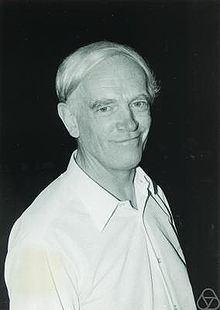
\includegraphics[width=0.3\textwidth]{./figures/Witt}
	\caption{Ernst Witt}
\end{figure}
\paragraph{Ernst Witt} % (fold)
\label{par:ernst_witt}
Ernst Witt\index{Ernst Witt} (June 26, 1911--July 3, 1991) was a German mathematician, one of the leading algebraists of his time. Witt completed his Ph.D. at the University of G\"{o}ttingen in 1934 with Emmy Noether. Witt's work has been highly influential. His invention of the Witt vectors clarifies and generalizes the structure of the $p$-adic numbers. It has become fundamental to $p$-adic Hodge theory. For more information, see \url{https://en.wikipedia.org/wiki/Ernst_Witt} and \url{http://www-history.mcs.st-andrews.ac.uk/Biographies/Witt.html}.
% paragraph ernst_witt (end)

%
%
%
\section{$p$-Witt vectors} % (fold)
\label{sec:p_witt_vectors}
In this section we introduce $p$-Witt vectors. Witt vectors generalize the $p$-adics and we will see all $p$-Witt vectors over any commutative ring form a ring. 

From now on, fix a prime number $p$.
\begin{definition}
	A $p$-Witt vector\index{$p$-Witt vectors} over a commutative ring $R$ is a sequence $(X_0,X_1,X_2,\cdots)$ of elements of $R$.
\end{definition}
\begin{remark}
	If $R=\mathbb{F}_p$, any $p$-Witt vector over $\mathbb{F}_p$ is just a $p$-adic integer $a_0+a_1p+a_2p^2+\cdots$ with $a_i\in \mathbb{F}_p$.
\end{remark}
We introduce Witt polynomials in order to define ring structure on $p$-Witt vectors.
\begin{definition}
Fix a prime number $p$, let $(X_0,X_1,X_2,\cdots)$ be an infinite sequence of indeterminates. For every $n\geq 0$, define the $n$-th Witt polynomial
\[
	W_n(X_0,X_1,\cdots)=\sum_{i=0}^n p^iX_i^{p^{n-i}}=X_0^{p^n}+pX_1^{p^{n-1}}+\cdots+p^nX_n.
\]
\end{definition}
For example, $W_0=X_0,\ W_1=X_0^p+pX_1,\ W_2=X_0^{p^2}+pX_1^p+p^2X_2$.

Question: how can we add and multiple Witt vectors?
\begin{theorem}
Let $(X_0,X_1,X_2,\cdots)$, $(Y_0,Y_1,Y_2,\cdots)$ be two sequences of indeterminates. For every polynomial function $\Phi \in \mathbb{Z}[X,Y]$, there exists a unique sequence $(\varphi_0,\cdots, \varphi_n,\cdots)$ of elements of $\mathbb{Z}[X_0,\cdots,X_n,\cdots;Y_0,\cdots,Y_n,\cdots]$ such that
\[
 	W_n(\varphi_0,\cdots, \varphi_n,\cdots)=\Phi\big(W_n(X_0,\cdots),W_n(Y_0,\cdots)\big),\ n=0,1,\cdots.
 \] 
\end{theorem}
If $\Phi=X+Y$(resp. $XY$), then there exist $(S_1,\cdots,S_n,\cdots)$(``$S$'' stands for sum) and $(P_1,\cdots,P_n,\cdots)$ (``$P$'' stands for product) such that
\[W_n(X_0,\cdots,X_n,\cdots)+W_n(Y_0,\cdots,Y_n,\cdots)=W_n(S_1,\cdots,S_n,\cdots),\]
\[W_n(X_0,\cdots,X_n,\cdots)W_n(Y_0,\cdots,Y_n,\cdots)=W_n(P_1,\cdots,P_n,\cdots).\]

Let $R$ be a commutative ring, if $A=(a_0,a_1,\cdots)\in R^\N$ and $B=(b_0,b_1,\cdots)\in R^\N$ are $p$-Witt vectors over $R$, we define
\[A+B=(S_0(A,B),  S_1(A,B),\cdots),\quad AB=(P_0(A,B),  P_1(A,B),\cdots).\]
\begin{theorem}
The $p$-Witt vectors over any commutative ring $R$ form a commutative ring under the compositions defined above (called the ring of $p$-Witt vectors with coefficients in $R$, denoted by $W(R)$).
\end{theorem}
\begin{example}
We have
\[
\begin{array}{cc}
	S_0(A,B) =a_0+b_0	& P_0(A,B)=a_0b_0\\
	S_1(A,B) =a_1+b_1+\frac{a_0^p+b_0^p-(a_0+b_0)^p}{p}	& P_1(A,B)=b_0^pa_1+a_0^pb_1+pa_1b_1
	\end{array}
\]
\end{example}
\begin{theorem}
There is a ring homomorphism
\begin{align*}
W_*\colon W(R) &\longrightarrow R^\N \\
(X_0,X_1,\cdots,X_n,\cdots)&  \mapsto (W_0,W_1,\cdots,W_n,\cdots)
\end{align*}
\end{theorem}
\begin{proof}
Only need to check this map is a ring homomorphism: since
\[A+B=(S_0(A,B),S_1(A,B),\cdots ),\quad AB=(P_0(A,B),P_1(A,B),\cdots ),\]
by definition we have
\begin{align*}
W(A)+W(B)&=(W_0(A)+W_0(B),W_1(A)+W_1(B),\cdots)\\
&=\big(W_0(S_0(A,B),S_1(A,B),\cdots ),W_1(S_0(A,B),S_1(A,B),\cdots ),\cdots\big)\\
&=W(S_0(A,B),S_1(A,B),\cdots )=W(A+B).
\end{align*}
And similarly,
\begin{align*}
W(A)W(B)&=(W_0(A)W_0(B),W_1(A)W_1(B),\cdots)\\
& =\big(W_0(P_0(A,B),P_1(A,B),\cdots ),W_1(P_0(A,B),P_1(A,B),\cdots ),\cdots\big)\\
& =W(P_0(A,B),P_1(A,B),\cdots )=W(AB).
\end{align*}
Indeed, we only need to show $W_n(A)+W_n(B)=W_n(A+B)$ and $W_n(A)W_n(B)=W_n(AB)$ which are obviously true. (实际上就是为了使得这个是同态而定义出了$A+B$和$AB$。)
\end{proof}
\begin{example}
	\begin{enumerate}
		\item If $p$ is invertible in $R$, then $W(R)=R^\N$ --- the product of countable number of $R$.(if $p$ is invertible the homomorphism $W_*$ is an
isomorphism.)
		\item $W(\mathbb{F}_p)=\Z_{(p)}$ --- the ring of $p$-adic integers.
		\item $W(\mathbb{F}_{p^n})$ is an unramified extension of the ring of $p$-adic integers.
	\end{enumerate}
\end{example}

Note that the functions $P_k$ and $S_k$ are actually only involve the variables of index $\leqslant k$ of $A$ and $B$. In particular if we truncate all the vectors at the $k$-th entry, we can still add and multiply them.
\begin{definition}
Truncated $p$-Witt ring\index{truncated $p$-Witt ring} $W_k(R)=\{(a_0,a_1,\cdots,a_{k-1})| a_i\in R\}$ (also called the ring of Witt vectors of length $k$.\index{the ring of Witt vectors of length $k$})
\end{definition}
\begin{example}
	$W_1(R)=R$, $W(R)=\varprojlim W_k(R)$. Since $W_k(\mathbb{F}_p)=\Z/p^k\Z$, $W(\mathbb{F}_p)=\Z_{(p)}$.
\end{example}
	
% Now, if we regard $W$ as a functor from the category of commutative rings to itself, we can think the following maps are actually natural transformations. %现在有一个问题是$V$是不是环同态
\begin{definition}
We define two special maps as follows
\begin{itemize}
	\item The ``shift'' map $V\colon W(R)\longrightarrow W(R)$, $(a_0,a_1,\cdots) \mapsto (0,a_0,a_1,\cdots)$, this map is {\em additive}.
	\item When $char(R)=p$, the ``Frobenius'' map $F\colon W(R)\longrightarrow W(R)$, $(a_0,a_1,\cdots) \mapsto (a_0^p,a_1^p,\cdots)$, this is indeed a ring homomorphism.
\end{itemize}
\end{definition}
Firstly, we note that $W_k(R)=W(R)/V^kW(R)$, and if we consider $V\colon W_n(R)\hookrightarrow W_{n+1}(R)$ there are exact sequences
\[0\longrightarrow W_k(R)\overset{V^r}\longrightarrow W_{k+r}(R)\longrightarrow W_r(R) \longrightarrow 0, \quad \forall k,\,r.\]

The  map $V\colon  W(R)\longrightarrow W(R)$  is  additive: for it suffices to verify this when  $p$ is  invertible in  $R$,  and  in  that  case the homomorphism
$W_*\colon W(R)\longrightarrow R^\N$ transforms $V$ into the map which sends $(w_0,w_1,\cdots)$ to $(0,pw_0,pw_1,\cdots)$.
\[
\begin{tikzcd}
	W(R) \arrow[r,"V"] \arrow[d,"W_*"] & W(R) \arrow[d,"W_*"]\\
	R^\N \arrow[r]  & R^\N
\end{tikzcd}
\]
\[
\begin{tikzcd}
	(a_0,a_1,\cdots) \arrow[r,mapsto,"V"] \arrow[d,mapsto,"W_*"] & (0,a_0,a_1,\cdots) \arrow[d,mapsto,"W_*"]\\
	(a_0,a_0^p+pa_1,a_0^{p^2}+pa_1^p+p^2a_2,\cdots) \arrow[r,mapsto] \arrow[d,equal] & (0,pa_0,pa_0^p+p^2a_1,\cdots)\arrow[d,equal]\\
	(w_0,w_1,w_2,\cdots) \arrow[r,mapsto]& (0,pw_0,pw_1,\cdots)\\
\end{tikzcd}
\]
If $x\in R$, define a map
\begin{align*}
r\colon & R\longrightarrow W(R)\\
& x\mapsto (x,0,\cdots,0,\cdots)
\end{align*}
When $p$ is invertible in $R$, $W_*$ transforms $r$
into the mapping that $x \mapsto (x, x^p, \cdots , x^{p^n}, \cdots )$. 
\[
\begin{tikzcd}
	R \arrow[r] \arrow[d,"\id"] & W(R) \arrow[d,"W_*"]\\
	R \arrow[r]  & R^\N
\end{tikzcd}
\]
\[
\begin{tikzcd}
	x \arrow[r,mapsto] \arrow[d,equal] & (x,0,\cdots,0,\cdots) \arrow[d,mapsto,"W_*"]\\
	x\arrow[r,mapsto] & (x,x^p,\cdots,x^{p^n},\cdots)\\
\end{tikzcd}
\]
One deduces by the same reasoning as above the  formulas:
\begin{prop}
	\begin{align*}
	r(xy)&=r(x)r(y),\ x,y\in R\\
	(a_0,a_1,\cdots)&=\sum_{n=0}^\infty V^n(r(a_n)),\ a_i\in R\\
	r(x)(a_0,\cdots)&=(xa_0,x^pa_1,\cdots,x^{p^n}a_n,\cdots),\ x_i,a_i\in R.
	\end{align*}
\end{prop}
\begin{proof}
The first formula: put $r(x)r(y),\ r(xy)$ to $R^\N$, we get $(x,x^p,\cdots,x^{p^n},\cdots)(y,y^p,\cdots,y^{p^n},\cdots)$ and $(xy,(xy)^p,\cdots,(xy)^{p^n},\cdots)$.\\
The second formula: put $(a_0,a_1,\cdots)$ to $R^\N$, we get $(a_0,a_0^p+pa_1,a_0^{p^2}+pa_1^p+p^2a_2,\cdots)$\\
consider $V^i(r(a_i))$: put $r(a_i)$ to $R^\N$, we get $(a_i,a_i^p,\cdots,a_i^{p^n},\cdots)\in R^\N$, and $W_*$ transforms $V$ to the mapping $(w_0,w_1,\cdots,w_n,\cdots)\mapsto (0,pw_0,\cdots,pw_{n-1},\cdots)$, \\
now we put $(r(a_0))$ to $R^\N$, we get $(a_0,a_0^p,\cdots,a_0^{p^n},\cdots)$\\
put $V^1(r(a_1))$ to $R^\N$, we get $(0,pa_1,\cdots,pa_1^{p^{n-1}},\cdots)$\\
put $V^2(r(a_2))$ to $R^\N$, we get $(0,0,p^2a_2,\cdots,p^2a_2^{p^{n-2}},\cdots)$\\
put $V^i(r(a_i))$ to $R^\N$, we get $(\underbrace{0,0,\cdots,0}_{i\mbox{ terms}},p^ia_i,\cdots,p^ia_i^{p^{n-i}},\cdots)$\\
so put $\sum_n V^n(r(a_n))$ to $R^\N$, we get $(a_0,a_0^p+pa_1,\cdots)$.\\
We leave the proof of the last formula to readers.
\end{proof}
\begin{prop}
	\[VF=p=FV.\]
\end{prop}
\begin{proof}
It suffices to check this when $R$ is perfect. Note that a ring $R$ of characteristic $p$ is called perfect if $x\mapsto x^p$ is an automorphism. For more details, we refer to page 44 on Serre's book {\em Local Fields}.
\end{proof}

% section p_witt_vectors (end)
\section{Big Witt vectors} % (fold)
\label{sec:big_witt_vectors}
Now we turn to the \texttt{big}(universal) Witt vectors\index{big Witt vectors}. J.\,P,\ May once said ``This(the theory of Witt vectors) is a strange and beautiful piece of mathematics that every well-educated mathematician should see at least once''.

Take the ring of all big vectors of a commutative ring is a functor 
\begin{align*}
\mathbf{CRing} &\longrightarrow \mathbf{CRing}\\
 R &\mapsto W(R).
\end{align*}
In this section, $R$ is a commutative ring with unit.
\begin{definition}
The ring of all big Witt vectors in $R$ which also denoted by $W(R)$ is defined as follows,\\
as a set: $W(R)=\{a(T)\in R[[T]]| a(T)=1+a_1T+a_2T^2+\cdots\}=1+TR[[T]]$; (we note that as a set $W(R)$ is the kernel of the map $A[[T]]^*\overset{T\mapsto 0}\longrightarrow A^*$)\\
addition in $W(R)$: usual multiplication of formal power series, sum $a(T)b(T)$, difference $\frac{a(T)}{b(T)}$;($(W(R),+)\cong (1+TR[[T]],\times)$ which is a subgroup of the group of units $R[[T]]^{\times}$ of the ring $R[[T]]$)\\
multiplication in $W(R)$: denoted by $*$, this is a little mysterious, we will talk the details later. For the present purposes we only define $*$ as the unique continuous functorial operation for which $(1-aT)*(1-bT)=(1-abT)$.\\
'zero'(additive identity) of $W(R)$: $1$.\\
'one'(multiplicative identity) of $W(R)$: $[1]=1-T$. Note that $[1]$ is the image of $1\in R$ under the multiplicative (Teichmuller) map 
\[R\longrightarrow W(R)\]
\[a \mapsto [a]=1-aT\]
functoriality: any homomorphism $f\colon R \longrightarrow S$ induces a ring homomorphism 
$W(f)\colon W(R) \longrightarrow W(S)$.
\end{definition}
A quick way to check multiplicative formulas in $W(R)$ is to use the \texttt{ghost} map\index{ghost map} (indeed a ring homomorphism)
\[gh\colon W(R)\longrightarrow R^\N =\prod_i^\infty R. \]
It is obtained from the abelian group homomorphism
\begin{align*}
-T \frac{d}{dT}\log \colon& (1+TR[[T]])^{\times} \longrightarrow (TR[[T]])^+\\
& a(T)\mapsto -T \frac{a'(T)}{a(T)}
\end{align*}
the right side of $gh$ is $R^\N$ via $\sum a_nt^n \longleftrightarrow (a_1,a_2,\cdots)$.

A basic principle of the theory of Witt vectors is that to demonstrate certain equations it suffices to check them on vectors of the form $1-aT$.
% section big_witt_vectors (end)
\section{Module structure on $NK_*$} % (fold)
\label{sec:module_structure_on_}
\paragraph{Notations} $\Lambda$: a ring with $1$\\
$R$: commutative ring \\
$W(R)$: the ring of big Witt vectors of $R$\\
$\mathbf{End}(\Lambda)$: the exact category of endomorphisms of finitely generated projective right $\Lambda$-modules.\\
$\mathbf{Nil}(\Lambda)$: the full exact subcategory of nilpotent endomorphisms.\\
$\mathbf{P}(\Lambda)$: the exact category of finitely generated projective right $\Lambda$-modules.

The fundamental theorem in algebraic $K$-theory states that
\[K_i(\Lambda[t])\cong K_i(\Lambda)\oplus NK_i(\Lambda)\cong K_i(\Lambda)\oplus \Nil_{i-1}(\Lambda),\]
and hence $\Nil(\Lambda)$ is the obstruction to $K$-theory being homotopy invariant. By a theorem of Serre, a ring $\Lambda$ is regular, if and only if every (right) $\Lambda$-module has a finite projective resolution. So the resolution theorem and the fact that $G$-theory is homotopy invariant show that for a regular ring, $NK_
*(\Lambda)=\Nil_{*-1}(\Lambda) = 0$. In general, one knows that the groups $\Nil_*(\Lambda)$, if non-zero, are infinitely generated. It is also known that the groups $\Nil_*(\Lambda)$ are modules over the big Witt ring $W(R)$ (just this notes want to show you).

Goals:
\begin{itemize}
	\item Define the $\End_0(R)$-module structure on $NK_*(\Lambda)$ 
	\item (Stienstra's observation) this can extend to a $W(R)$-module structure.
	\item Computations in $W(R)$ with Grothendieck rings.
\end{itemize}
\subsection{$\End_0(\Lambda)$}\index{$\End_0(\Lambda)$}
Let $\mathbf{End}(\Lambda)$ denote the exact category of endomorphisms of finitely generated projective right $\Lambda$-modules.\\
Objects: pairs $(M,f)$ with $M$ finitely generated projective and $f\in \End(M)$.\\
Morphisms: $(M_1,f_1) \overset{\alpha}\longrightarrow (M_2,f_2)$ with $f
_2\circ \alpha =\alpha \circ f_1$, i.e. such $\alpha$ make the following diagram commutes
\[
\begin{tikzcd}
	M_1 \arrow[r,"f_1"] \arrow[d,"\alpha"] & M_1 \arrow[d,"\alpha"]\\
	M_2 \arrow[r,"f_2"]  & M_2
\end{tikzcd}
\]
There are two interesting subcategories of $\mathbf{End}(\Lambda)$ --- \\
$\mathbf{Nil}(\Lambda)$: the full exact subcategory of nilpotent endomorphisms.\\
$\mathbf{P}(\Lambda)$: the exact category of finitely generated projective right $\Lambda$-modules. (Remark: the reflective subcategory of zero endomorphisms is natually equivalent to $\mathbf{P}(\Lambda)$. Note that a full subcategory $i\colon \mathcal{C} \longrightarrow \mathcal{D}$ is called reflective if the inclusion functor $i$ has a left adjoint $T$, $(T \dashv i) \colon \mathcal{C}  \rightleftarrows \mathcal{D}$.)

Since inclusions are split and all the functors below are exact, they induce homomorphisms between $K$-groups
\[\mathbf{P}(\Lambda)  \rightleftarrows \mathbf{Nil}(\Lambda)\]
\[\mathbf{P}(\Lambda)  \rightleftarrows \mathbf{End}(\Lambda)\]
\[M \mapsto (M,0)\]
\[M \mapsfrom (M,f)\]
\begin{definition}
	$K_n(\mathbf{End}(\Lambda))=K_n(\Lambda) \oplus \End_n(\Lambda)$, $K_n(\mathbf{Nil}(\Lambda))=K_n(\Lambda) \oplus \Nil_n(\Lambda)$
\end{definition}
Now suppose $\Lambda$ is an $R$-algebra for some commutative ring $R$, then there are exact pairings (i.e. bifunctors):
\begin{align*}
	\otimes\colon &\mathbf{End}(R) \times \mathbf{End}(\Lambda) \longrightarrow \mathbf{End}(\Lambda) \\
	\otimes\colon &\mathbf{End}(R) \times \mathbf{Nil}(\Lambda) \longrightarrow \mathbf{Nil}(\Lambda) \\
 				  & (M,f) \otimes (N,g)=(M\otimes_R N, f\otimes g)
\end{align*}
These induce (use ``generators-and-relations'' tricks on $K_0$)
\begin{align*}
	K_0(\mathbf{End}(R)) \otimes K_*(\mathbf{End}(\Lambda)) \longrightarrow K_*(\mathbf{End}(\Lambda)) \\
	K_0(\mathbf{End}(R)) \otimes K_*(\mathbf{Nil}(\Lambda)) \longrightarrow K_*(\mathbf{Nil}(\Lambda)) \\
\end{align*}
$[(0,0)], [(R,1)]\in K_0(\mathbf{End}(R))$ act as the zero and identity maps.

I think we can fix an element $(M,f)\in \mathbf{End}(R)$, then $(M,f)\otimes$ induces an endofunctor of $\mathbf{End}(\Lambda)$. We can get endomorphisms of $K$-groups, then we check that this does not depent on the isomorphism classes and the bilinear property. (Can also see Weibel The $K$-book chapter2, chapter3 Cor 1.6.1, Ex 5.4, chapter4 Ex 1.14.)

If we take $R = \Lambda$, we see that $K_0(\mathbf{End}(R))$ is a commutative ring with unit $[(R,1)]$. $K_0(R)$ is an
ideal, generated by the idempotent $[(R,0)]$, and the quotient
ring is $\End_0(R)$.  Since $(R,0)\otimes$ reflects $\mathbf{End} (\Lambda)$ into $\mathbf{P} (\Lambda)$,
\[i\colon \mathbf{P} (\Lambda) \longrightarrow \mathbf{End} (\Lambda);\quad
 (R,0)\otimes\colon \mathbf{End} (\Lambda) \longrightarrow \mathbf{P} (\Lambda)\]
$K_0(R)$ acts as zero on $\End_*(\Lambda)$ and $\Nil_*(\Lambda)$. (Consider $P\in \mathbf{P}(R)$ acts on $\mathbf{End}(\Lambda)$, $(P,0)\otimes (N,g)=(P\otimes_R N,0) \in \mathbf{P}(\Lambda)$. )

The following is immediate (and well-known):
\begin{prop}\label{endmodule}
	If  $\Lambda$ is an $R$-algebra with $1$, $\End_*(\Lambda)$ and
$\Nil_*(\Lambda)$ are graded modules over the ring $\End_0 (R)$.
\end{prop}
Now we focus on $*=0$ and $\Lambda =R$:\\

The inclusion of $\mathbf{P}(R)$ in $\mathbf{End}(R)$ by $f = 0$ is split by the forgetful functor, and the kernel $\End_0 (R)$ of $K_0\mathbf{End}(R) \longrightarrow K_0 (R)$ is not only an ideal but a commutative ring with unit $1 = [(R,1)] - [(R, 0)]$.

\begin{theorem}[Almkvist]\label{Almkvist}
The homomorphism (in fact it is a ring homomorphism)
\begin{align*}
	\chi \colon&  \End_0(R)\longrightarrow W(R)=(1+TR[[T]])^{\times}\\
     & (M,f) \mapsto \det(1-fT)
\end{align*}
	is injective and $\End_0(R)\cong \ima \chi =\left\{\frac{g(T)}{h(T)}\in W(R)\mid g(T),h(T) \in 1+TR[T]\right\}$
\end{theorem}
The map $\chi$ (taking characteristic polynomial\index{characteristic polynomial}) is well-difined, and we have 
\[\chi([(R,0)])=1, \quad \chi([(R,1)])=1-T\]
$\chi$ is a ring homomorphism, and $\ima \chi =$ the set of all rational functions in $W(R)$. Note that 
\[\det (1-fT)\det(1-gT)=\det(1-(f\oplus g)T),\quad \det (1-fT)*\det(1-gT)=\det(1-(f\otimes g)T),\]
for more details we refer the reader to S.Lang {\em Algebra}, Chapter 14, Exercise 15.
\begin{remark}
	when $R$ is a algebraically closed field (for instance $\mathbb{C}$), we can use Jordan canonical forms to prove the last identity (i.e. it can be reduced to check that $\prod_i (1-\lambda_i T) * \prod_j (1-\mu_j T) =\prod_{i,j} (1-\lambda_i \mu_j T)$).
\end{remark}


\begin{definition}[$NK_*$]
	As above, we define $NK_n(\Lambda)=\ker(K_n(\Lambda[y])\longrightarrow K_n(\Lambda))$. Grayson proved that $NK_n(\Lambda)\cong \Nil_{n-1}(\Lambda)$ in ``Higher algebraic $K$-theory II''. The map is given by 
	\[NK_n(\Lambda) \subset K_n(\Lambda[y]) \subset K_n(\Lambda[x,y]/xy=1)\overset{\partial}\longrightarrow K_{n-1}(\mathbf{Nil}(\Lambda)).\]
	Thus $NK_n(\Lambda)$ are $\End_0(R)$-modules. For $n \geq 1$, this is just \ref{endmodule}; for $n = 0$ (and $n < 0$) this follows from the functoriality of the module structure and the fact that $NK_0(\Lambda)$ is the ``contracted functor'' of $NK_1(\Lambda)$.
\end{definition}

Note that $NK_1(\Lambda)\cong K_1(\Lambda[y],(y-\lambda))$, $\forall \lambda\in \Lambda$, since 
\begin{gather*}
	\Lambda[y] \rightleftarrows \Lambda\\
y\mapsto \lambda.
\end{gather*}
Since $[(P,\nu)]=[(P\oplus Q,\nu\oplus 0)]-[(Q,0)]\in K_0(\mathbf{Nil}(\Lambda))$, we see $\Nil_0(\Lambda)$ is generated by elements of the form $[(\Lambda^n,\nu)]-n[(\Lambda,0)]$ for some $n$ and some nilpotent matrix $\nu$
Sign convention:
\begin{align*}
	NK_1(\Lambda) & \cong \Nil_0(\Lambda)\\
[1-\nu y] & \leftrightarrow [(\Lambda^n,\nu)]-n[(\Lambda,0)]
\end{align*}
\begin{example}
	Let $k$ be a field, $\mathbf{End}(k)$ consists pairs $(V,A)$ with $V$ a finite-dimensional vector space over $k$ and $A$ a $k$-endomorphism. Two pairs are isomorphic if and only if their minimal polynomials are equal. When we consider $\mathbf{Nil}(k)$, then $K_0(\mathbf{Nil}(k))\cong \mathbb{Z}$, we conclude that $\Nil_0(k)=0$. Recall that since $k$ is a regular ring, $NK_*(k)=0$, we have another proof of $NK_1(k)\cong \Nil_0(k)=0$.
\end{example}


\subsection{Grothendieck rings and Witt vectors}
\label{subsec:grothendieck_rings_and_witt_vectors}
We refer the reader to Grayson's paper {\em Grothendieck rings and Witt vectors}.
\begin{definition}
	A $\lambda$-ring $R$\index{$\lambda$-ring} is a commutative  ring with $1$, together with an operation $\lambda_t$ which assigns to each element $x$ of $R$ a power series
	\[\lambda_t(x)=1+\lambda^1(x)t+\lambda^2(x)t^2+\cdots, \quad x\in R\]
	This operation must obey $\lambda_t(x+y)=\lambda_t(x)\lambda_t(y)$. 
\end{definition}
Let $R$ is a commutative ring with unit, $K_0(R)=K_0(\mathbf{P}(R))$ becomes a $\lambda$-ring if we define 
\[[M][N]=[M\otimes_R N], \quad \lambda_t^n([M])=[\wedge^n_R M]. \]
Recall $M\otimes_R(N\oplus N')\cong (M\otimes_R N)\oplus(M\otimes_R N')$, $\wedge^n(M\oplus M')\cong \bigoplus_{i+j=n}\wedge^i M\otimes \wedge^j M'$, and $\wedge^n(M):=M^{\otimes n}/\langle x\otimes x \mid x\in M\rangle$, $\rank \wedge^n(M)=\binom{\rank M}{n}. $

For instance, if $R$ is a field, $K_0(R)=\Z$ and $\lambda_t(n)=(1+t)^n=1+\binom{n}{1}t+\binom{n}{2}t^2+\cdots+\binom{n}{n}t^n$, since $\dim (\wedge^i R^n)=\binom{n}{i}$.

We make $K_0(\mathbf{End}(R))$ into a $\lambda$-ring by defining
\[\lambda^n([M, f])=([\wedge^n M,\wedge^n f]).\]
The ideal generated by the idempotent $[(R,0)]$ is isomorphic to $K_0(R)$, the quotient $\End_0(R)$ is a $\lambda$-ring. It is convenient to think of $\End_0$ as a convariant functor on the category of rings, and the functor $\End_0$ satisfies:
\begin{enumerate}
	\item If $R\longrightarrow S$ is surjective ring homomorphism, then $\End_0(R)\longrightarrow \End_0(S)$ is surjective.
	\item If $R$ is an algebraically close field, then the group $\End_0(R)$ is generated by the elements of the form $[(R,r)]$. (This holds because any matrix over $R$ is triagonalizable.)
\end{enumerate}

Recall 
\begin{align*}
	\chi \colon&  \End_0(R)\longrightarrow W(R)=1+TR[[T]]\\
     & (M,f) \mapsto \det(1-fT)
\end{align*}
$W(R)$ is the underlying (additive) group of the ring of Witt vectors. The $\lambda$-ring operations on $W(R)$ are the unique operations which are continuous, functorial in $R$, and satisfy:
\begin{gather*}
	(1-aT)*(1-bT)=1-abT\\
	\lambda_t(1-aT)=1+(1-aT)t
\end{gather*}

By \ref{Almkvist}, $\chi$ is an injective ring homomorphism whose image consists of all Witt vectors which are quotients of polynomials. In fact $\chi$ is a $\lambda$-ring homomorphism, so we have
\begin{theorem}
	$\End_0(R)$ is dense sub-$\lambda$-ring of $W(R)$.
\end{theorem}
	The hard part of the theorem is the injectivity. When $R$ is a field the injectivity follows immediately from the existence of the rational canonical form (we can see it below) for a matrix. The result is surprising when $R$ is not a field.
\paragraph{Computation in $W(R)$}
Computation in $W(R)$ which is tedious unless we perform it in $\End_0(R)$:
\[(1-aT^2)*(1-bT^2)=?\]
Note that $\chi\Big(\begin{pmatrix}
	0&a \\1&0
\end{pmatrix}\Big)=\det \begin{pmatrix}
	1&-aT\\-T &1
\end{pmatrix} =1-aT^2$, $\chi\Big(\begin{pmatrix}
	0&b \\1&0
\end{pmatrix}\Big)=\det \begin{pmatrix}
	1&-bT\\-T &1
\end{pmatrix} =1-bT^2$,
\begin{gather*}
	\chi\Big(\begin{pmatrix}
	0&a \\1&0
\end{pmatrix}\Big)*\chi\Big(\begin{pmatrix}
	0&b \\1&0
\end{pmatrix}\Big)=\chi\Big(\begin{pmatrix}
	0&a \\1&0
\end{pmatrix}\otimes \begin{pmatrix}
	0&b \\1&0
\end{pmatrix} \Big)=\chi \Big(\begin{pmatrix}
	0 &0&0&ab\\0&0&b&0\\0&a&0&0\\1&0&0&0
\end{pmatrix}\Big)\\
=\det \begin{pmatrix}
	1 &0&0&-aTb\\0&1&-bT&0\\0&-aT&1&0\\-T&0&0&1
\end{pmatrix}=1-2abT^2+a^2b^2T^4.
\end{gather*}

If we use the previous formula 
\[(1-rT^m)*(1-sT^n)=(1-r^{n/d}s^{m/d}T^{mn/d})^d,\ d=\mbox{gcd}(m,n),\]
we obtain the same answer. Indeed we have the formula 
\[\det (1-fT)*\det(1-gT)=\det(1-(f\otimes g)T),\]
if a polynomial is $1 + a_1T+ \cdots + a_nT^n\in W(R)$, we can write $f=\begin{pmatrix}
	0& & & & -a_n\\
	1&0& & & -a_{n-1}\\
	 &\ddots&\ddots& &\vdots\\
	 & & 1&0&-a_2\\
	 & & & 1&-a_1 
\end{pmatrix}\in M_n(R)$.

\paragraph{Operations on $W(R)$ and $\End_0(R)$}
We have already known that $W$ and $\End_0$ can be regarded as functors from the category of commutative rings to that of ($\lambda$-)rings. The following operations $F_n,\  V_n \colon W \Longrightarrow W (\mbox{resp. }\End_0 \Longrightarrow \End_0) $ are indeed natural transformation.
These auxiliary operations defined on $W(R)$ can also be computed in $\End_0(R)$.
\begin{enumerate}
	\item the ghost map \index{ghost map}
	\[gh \colon W(R) \xrightarrow{-T\frac{d}{dT}\log} TR[[T]] \cong R^{\N},\quad \alpha(T)\mapsto \frac{-T}{\alpha(T)} \frac{d\alpha}{d T}. \] 
	and  the $n$-th ghost coordinate \index{ghost coordinates}
	\[gh_n \colon W(R)\longrightarrow R\]
	it is the unique continuous natual additive map which sends $1-aT$ to $a^n$.

	Remark. $gh(1-aT)=\frac{aT}{1-aT}=\sum_{i=1} a^iT^i$.The exponential map is defined by
	\[R^{\N}\longrightarrow W(R),\quad (r_1,\cdots) \mapsto \prod_{i=1}^\infty \exp (\frac{-r_i T^i}{i}). \]
	

	\item the Frobenius endomorphism
	\[F_n \colon W(R)\longrightarrow W(R),\quad \alpha(T)\mapsto \sum_{\zeta^n=1}\alpha(\zeta T^{\frac{1}{n}}). \]
	it is the unique continuous natual additive map which sends $1-aT$ to $1-a^nT$.

	Remark. $F_n(1-aT)=\sum_{\zeta^n=1}(1-a\zeta T^{\frac{1}{n}})=1-a^nT $, since ``$+$'' in $W(R)$ is the normal product.

	\item the Verschiebung endomorphism
	\[V_n \colon W(R)\longrightarrow W(R),\quad \alpha(T)\mapsto \alpha(T^n). \]
	it is the unique continuous natual additive map which sends $1-aT$ to $1-aT^n$.
\end{enumerate}
\begin{equation*}
	\begin{array}{c|l|c}
	\mbox{ghost map } gh_n\colon W(R)\longrightarrow R & 1-aT \mapsto a^n & \\
	\hline
	\mbox{Frobenius endomorphism } F_n \colon W(R)\longrightarrow W(R)&  1-aT\mapsto 1-a^nT & \alpha(T)\mapsto \sum_{\zeta^n=1}\alpha(\zeta T^{\frac{1}{n}}) \\
	\hline
	\mbox{Verschiebung endomorphism }V_n \colon W(R)\longrightarrow W(R) &1-aT\mapsto 1-aT^n&\alpha(T)\mapsto \alpha(T^n)
\end{array}
\end{equation*}

We define similar operations on $\End_0(R)$ as follows:
\begin{equation*}
	\begin{array}{c|l}
	 gh_n\colon \End_0(R) \longrightarrow R & [(M,f)] \mapsto \tr(f^n)  \\
	\hline
	 F_n \colon \End_0(R) \longrightarrow \End_0(R) &  [(M,f)]\mapsto [(M,f^n)]  \\
	\hline
	V_n \colon \End_0(R) \longrightarrow \End_0(R)  &[(M,f)]\mapsto [(M^{\oplus n},v_nf)]
\end{array}
\end{equation*}
where $v_nf$ is represented by $\begin{pmatrix}
	0& &  &f\\1&0 & &\\ &\ddots&\ddots&\\ & &1&0
\end{pmatrix}$. The matrix $v_nf$ is close to an $n$-th root of $f$. Another equivalent description is
\[V_n\colon [(M,f)] \mapsto [(M[y]/y^n-f,y)].\]
% $\begin{pmatrix}
% 	0& & & &f\\1&0& & &\\ &1&\ddots& &\\ & &\ddots &0 & \\ & & &1&0
% \end{pmatrix}$  %这是个写出来大的矩阵

One easily checks that the operations just defined are additive with respect to short exact sequences in $\mathbf{End}(R)$, and thus are well-defined on $\End_0(R)$.

Since $\End_0(R) \subset W(R)$ is dense and $gh_n,\ F_n,\ V_n$ are continuous, identities among them may be verified on $W(R)$ by checking them on $\End_0(R)$.  
\begin{equation*}
	\begin{array}{ccc}
	W(R) &\longleftrightarrow &\End_0(R)\\
	\hline
	 gh_n(v*w)=gh_n v*gh_n w  & & \tr((f\otimes g)^n)=\tr(f^n)\tr(g^n)\\
	 F_n(v*w)=F_n v*F_n w & &  (f\otimes g)^n=f^n\otimes g^n  \\	
	F_nV_n=n &  & (v_nf)^n=\begin{pmatrix}
 f & & \\ &\ddots & \\ & & f		
	\end{pmatrix} \\
	gh_nV_d(v)=\begin{cases}
		d\,gh_{n/d}(v), \mbox{ if }d\mid n \\0, \mbox{ if } d\nmid n
	\end{cases} & & \tr((v_d f)^n)=\begin{cases}
		d\,\tr(f^{n/d}), \mbox{ if }d\mid n \\0, \mbox{ if } d\nmid n
	\end{cases}
\end{array}
\end{equation*}
From the last row we may recover the usual expression of the ghost coordinates\index{ghost coordinates} in terms of the Witt coordinates \index{Witt coordinates}. The Witt coordinates of a vector $v$ are the coefficients in the expression
\[v=\prod_{i=1}(1-a_iT^i)=\prod_{i=1}V_i(1-a_i T). \]
We obtain
\[gh_n(v)=\sum_{d\mid n}da_d^{n/d}. \]

``Many mordern treatments of the subject of Witt vectors take this latter expression as the starting point of the theory.''

The logarithmic derivative of $1-a_dT^d$ is $\frac{d}{dT}\log (1-a_dT^d)=-\sum_{m=1}^\infty da_d^mT^{dm-1}$, and $-T\frac{d}{dT}\log (1-a_dT^d)=\sum_{n=1}^\infty gh_n(1-a_dT^d) T^n$. So we obtain the formula:
\[-Tv^{-1}\frac{dv}{dT}=\sum_{n=1}^\infty gh_n(v)T^n\]
which yields the exponential trace formula:
\[-T\chi([M,f])^{-1}\frac{d\chi([M,f])}{dT}=\sum_{n=1}^\infty \tr(f^n)T^n.\]
For example, when $\rank M =2$, we have $\tr(f^2)=(\tr(f))^2-2\det(f)$, note that $\det(1-fT)=1-\tr(f)T+\det(f)T^2$.

\begin{remark}
	When $R$ is a field, the exponential trace formula 
	\[-T\frac{d}{dT}\log \det(1-fT)=\sum_{n=1}^\infty \tr(f^n)T^n\]
	can be checked by $\det(1-fT)=\prod (1-\lambda_i T)$ where $\lambda_i$ are eigenvalues. And we also have
	\[\det(1-fT)=\exp(\sum_{n=1}^\infty -\tr(f^n)\frac{T^n}{n}),\]
	since $\prod (1-\lambda_i T)=\exp \big(\ln(\prod (1-\lambda_i T))\big)=\exp\big(\sum \ln (1-\lambda_i T)\big)$ and recall that formally $\ln(1-x) = -\sum \frac{x^n}{n}$.
\end{remark}



%
% $\End_0(R)$-module structure on $\Nil_0(\Lambda)$
%
\subsection{$\End_0(R)$-module structure on $\Nil_0(\Lambda)$}
Recall $\Lambda$ is an $R$-algebra, where $R$ is a commutative ring with unit. We define a map
\begin{align*}
	\End_0(R)\times \Nil_0(\Lambda) \longrightarrow \Nil_0(\Lambda) \\
	(R^n,f)*[(P,\nu)]=[(P^n,f\nu)]
\end{align*}

Let $\alpha_n=\alpha_n(a_1,\cdots,a_n)$ denote the $n\times n$ matrix (looks like the rational canonical form) over $R$:
\[\alpha_n(a_1,\cdots,a_n)=\begin{pmatrix}
	0& & & & -a_n\\
	1&0& & & -a_{n-1}\\
	 &\ddots&\ddots& &\vdots\\
	 & & 1&0&-a_2\\
	 & & & 1&-a_1 
\end{pmatrix}\]
Recall
\begin{align*}
	\chi \colon&  \End_0(R)\rightarrowtail W(R) \\
	 & (R^n,\alpha_n) \mapsto \det(1-\alpha_n T)
\end{align*}
we obtain
\[\det \begin{pmatrix}
	1& & & & a_n T\\
	-T&1& & & a_{n-1} T\\
	 &\ddots&\ddots& &\vdots\\
	 & & -T&1&a_2 T\\
	 & & & -T&1+a_1 T 
\end{pmatrix}=1+a_1T+\cdots+a_nT^n\]
(Computation methods: 1. the traditional computation. 2. Note that if $A$ is invertible,
\[\det \begin{pmatrix}
	A &B \\ C& D
\end{pmatrix} =\det(A)\det(D-CA^{-1}B).\]
In this case $A^{-1}=\begin{pmatrix}
	1& & & & \\
	T&1& & & \\
	 \vdots&\ddots&\ddots& &\\
	 T^{n-3}& \cdots& T&1&\\
	 T^{n-2}&T^{n-3} &\cdots & T&1 
\end{pmatrix}$)

Then we can also conclude that $\ima \chi =\left\{\frac{g(T)}{h(T)}\in W(R)\mid g(T),h(T) \in 1+TR[T]\right\}$.
{\color{red}
\begin{remark}
	Why is a general elment of the form $(R^n,\alpha_n)$? Namely how to reduce an endomorphism to a rational canonical form ?
\end{remark}}
Now we want to check some identities
\begin{gather*}
	\End_0(R)\times \Nil_0(\Lambda) \longrightarrow \Nil_0(\Lambda) \\
	(R^n,\alpha_n )*[(P,\nu)]=[(P^n,\alpha_n \nu)] \quad \mbox{by definition}\\
	(R^{n+1},\alpha_{n+1}(a_1,\cdots,a_n,0))*[(P,\nu)]=(R^n,\alpha_n )*[(P,\nu)] \quad \mbox{compute under $\chi$}\\
	(R^n,\alpha_n )*[(P,\nu)]=[(P^n,\beta)] \quad \mbox{where $\beta=\alpha_n(a_1\nu,\cdots,a_n\nu^n)$}
\end{gather*}
In fact, the last identity always holds when $R=\Z[a_1,\cdots,a_n]$. $\beta$ is nilpotent because $\beta =\alpha_n\nu$.

We only show how to check the last equation: only need to show that 
$$\alpha_n \nu =\alpha_n(a_1\nu,\cdots,a_n\nu^n)$$
\[LHS=\begin{pmatrix}
	0& & & & -a_n\nu\\
	\nu &0& & & -a_{n-1}\nu\\
	 &\ddots&\ddots& &\vdots\\
	 & & \nu &0&-a_2\nu\\
	 & & & \nu &-a_1\nu 
\end{pmatrix},\quad RHS=\begin{pmatrix}
	0& & & & -a_n\nu^n\\
	1&0& & & -a_{n-1}\nu^{n-1}\\
	 &\ddots&\ddots& &\vdots\\
	 & & 1&0&-a_2\nu^2\\
	 & & & 1&-a_1\nu 
\end{pmatrix}\]
we can check this using the characteristic polynomial since $\chi$ is injective: check
\[\det (1-\alpha_n \nu T) = \det (1-\alpha_n(a_1\nu,\cdots,a_n\nu^n)T)\]
\[LHS=\det \begin{pmatrix}
	1& & & & a_n \nu T\\
	-\nu T&1& & & a_{n-1} \nu T\\
	 &\ddots&\ddots& &\vdots\\
	 & & -\nu T&1&a_2 \nu T\\
	 & & & -\nu T&1+a_1 \nu T 
\end{pmatrix}=\det(1+a_1\nu T+\cdots+a_n\nu^nT^n)\]
\[RHS=\det \begin{pmatrix}
	1& & & & a_n\nu^n T\\
	-T&1& & & a_{n-1}\nu^{n-1} T\\
	 &\ddots&\ddots& &\vdots\\
	 & & -T&1&a_2\nu^2 T\\
	 & & & -T&1+a_1 \nu T
\end{pmatrix}=\det(1+a_1\nu T+\cdots+a_n\nu^nT^n).\]

Note that if $\exists N$ such that $\nu^N=0$, $\beta$ is independent of the $a_i$ for $i\geq N$. If $\nu^N =0$ then $\alpha_n \otimes \nu$ represents $0$ in $\Nil_0(\Lambda)$ whenever $\chi(\alpha_n)\equiv 1 \bmod t^N$.

\paragraph{More operations} 
Let $F_n\mathbf{Nil}(\Lambda)$ denote the full exact subcategory of $\mathbf{Nil}(\Lambda)$ on the $(P, \nu)$ with $\nu^n = 0$. If $\Lambda$ is an algebra over a commutative
ring $R$, the kernel $F_n\Nil_0(\Lambda)$ of $K_0 (F_n\mathbf{Nil}(\Lambda)) \longrightarrow  K_0 (\mathbf{P}(\Lambda))$ is an $\End_0(R)$-module and $F_n\Nil_0(\Lambda)\longrightarrow \Nil_0(\Lambda)$ is a module map.

The exact endofunctor $F_m \colon (P, \nu)\mapsto  (P, \nu^m)$ on $\mathbf{Nil}(\Lambda)$ is zero on $F_m\mathbf{Ni1}(\Lambda)$. For $\alpha \in \End_0(R)$ and $(P, \nu) \in \Nil_0(\Lambda)$, nota that $(V_m \alpha)*(P, \nu) =
V_m (\alpha *F_m (P, \nu))$, and we can conclude that $V_m \End_0(R)$ acts trivially on the image of $F_m \Nil_0(\lambda)$ in $\Nil_0(\lambda)$. For more details, see Weibel, $K$-book chapter 2, pp 155 Exercise II.7.17.




%
%$W(R)$-module structure on $\Nil_0(\Lambda)$
%
\subsection{$W(R)$-module structure on $\Nil_0(\Lambda)$}
Once we have a nilpotent endomorphism, we can pass to infinity.
\begin{theorem}
	$\End_0(R)$-module structure on $\Nil_0(\Lambda)$ extends to a $W(R)$-module structure by the formula
	\[(1+\sum a_iT^i)*[(P,\nu)]=(R^n,\alpha_n(a_1,\cdots,a_n))*[(P,\nu)], \ n \gg 0.\]
\end{theorem}

% 
% $W(R)$-module structure on $\Nil_*(\Lambda)$
%
\subsection{$W(R)$-module structure on $\Nil_*(\Lambda)$}
The induced $t$-adic topology on $\End_0(R)$ is defined by the ideals 
\[I_N = \{f \in \End_0(R) \mid \chi(f) \equiv 1\bmod t^N\}, \ I_N\supset I_{N+1},\] 
and $\End_0 (R)$ is separated (i.e.\ $\cap I_N =0$) in this topology.  The key fact is:
\begin{theorem}[Almkvist]
	The map $\chi \colon \End_0 (R) \longrightarrow W(R)$ is a ring injection, and $W(R)$ is the $t$-adic completion of $\End_0 (R)$, i.e.\ $W(R)=\varprojlim \End_0(R)/I_N$.
\end{theorem}
\begin{theorem}[Stienstra]
	For every $\gamma \in \Nil_*(\Lambda)$ there is an  $N$ so that $\gamma$ is annihilated by the ideal
\[I_N = \{f \mid \chi(f)\equiv 1\bmod t^N\} \subset \End_0 (R).\]
Consequently, $NK_*(\Lambda)$ is a module over the $t$-adic completion $W(R)$ of $\End_0(R)$.
\end{theorem}

Recall the sign convention:
\begin{align*}
	NK_1(\Lambda) & \cong \Nil_0(\Lambda)\\
[1-\nu y] & \leftrightarrow [(\Lambda^n,\nu)]-n[(\Lambda,0)]
\end{align*}
The $W(R)$-module structure on $NK_1(\Lambda)$ is completely determined by the formula
\[\alpha(t) * [1-\nu y]=[\alpha(\nu y)].\]
And the $W(R)$-module structure on $NK_n(\Lambda)$ 
\[\alpha(t) * \{\gamma,1-\nu y\}=\{\gamma,\alpha(\nu y)\} \in NK_n(\Lambda), \quad \gamma\in K_{n-1}(R).\]
%
% Modern version
%
\subsection{Modern version}
Reference: Weibel, $K$-book, chapter 4, pp.\,58.
% section module_structure_on_ (end)

\section{Some results} % (fold)
\label{sec:some_results}
\begin{prop}
	If $R$ is $S^{-1}\Z,\hat{\Z_p}$ or $\Q$-algebra, then
	\begin{align*}
		\lambda_t \colon& R\longrightarrow W(R)\\
		& r\mapsto (1-t)^r
	\end{align*}
	is a ring injection.
\end{prop}
\begin{corollary}
	Fix an integer $p$ and a ring $\Lambda$ with $1$.\\
(a) If $\Lambda$ is an $S^{-1}\Z$-algebra, $NK_*(\Lambda)$ is an $S^{-1}\Z$-module.\\
(b) If $\Lambda$ is a $\Q$-algebra, $NK_*(\Lambda)$ is a  center($\Lambda$)-module.\\
(c) If $\Lambda$ is a $\hat{\Z_p}$-algebra, $NK_*(\Lambda)$ is a $\hat{\Z_p}$-module.\\
(d) If $p^m=0$ in $\Lambda$, $NK_*(\Lambda)$ is a $p$-group.
\end{corollary}
\begin{theorem}[Stienstra]
	If $0\neq n\in \Z$, $NK_1(R)[\frac{1}{n}]\cong NK_1(R[\frac{1}{n}])$.
\end{theorem}
\begin{corollary}\footnote{Weibel, $K$-book chapter3, page 27.}
	If $G$ is a finite group of order $n$, then $NK_1(\Z[G])$ is annihilated by some power of $n$. In fact, $NK_*(\Z[G])$ is an $n$-torsion group, and $Z_{(p)}\otimes NK_*(\Z[G])=NK_*(\Z_{(p)}[G])$, where $p\mid n$.
\end{corollary}
% section some_results (end)
 %Witt rings and NK_* groups
% \newcommand{\Ga}{\mathbf{G}_\mathrm{a}}
\newcommand{\Gm}{\mathbf{G}_\mathrm{m}}


\chapter{代数群}
主讲:魏达盛
\paragraph{2015.10.15}
\section{Affine linear algebraic groups}		
对于一般的代数群$G$,有以下正合列
\[0\longrightarrow G^{\mbox{aff}} \longrightarrow G\longrightarrow \mathbb{A} \longrightarrow 0\]
其中$G^{\mbox{aff}}$仿射代数群,$\mathbb{A}$是abelian variety.

\begin{definition}
	Affine algebraic groups\index{Affine algebraic groups}
\end{definition}
\begin{example}一些基本的例子如下
	\begin{itemize}
		\item[1] $\Ga$(additive group of $k$)\index{additive group of $k$,$\Ga$}: as a variety, $\Ga \cong \mathbb{A}^1$
		\[m \colon \mathbb{A}^1 \times \mathbb{A}^1 \longrightarrow \mathbb{A}^1\]
		\[(x,y) \mapsto x+y\]
		\item[2] $\Gm$(multiplicative group of $k$)\index{multiplicative group of $k$,$\Gm$}: as a variety, $\Gm \cong \mathbb{A}^1-\{0\}\cong \{xy-1=0\}\subset \mathbb{A}^2$
		\[m \colon \mathbb{A}^1-\{0\} \times \mathbb{A}^1-\{0\} \longrightarrow \mathbb{A}^1-\{0\}\]
		\[(x,y) \mapsto xy\]
		\[i \colon x \mapsto x^{-1}\]
		\item[3] The subgroup of $n$-th roots of unity of $\Gm$, denoted by $\bm{\mu}_n$: as a variety, $\bm{\mu}_n \cong \{x^n-1=0\}\subset\Gm$. 注:这里要求$\mbox{char}(k) \nmid n$,否则这个不是reduced variety.
		\item[4] Some classical group. The group of invertible matrices $\GL_n$ over $k$: as a variety $\GL_n \cong \{A \in M_n(k)=\mathbb{A}^{n^2}| \det (A) \neq 0\} \cong \{(A,y)\in M_n(k)\times \mathbb{A}^1 | \det(A)\cdot y=1\}$
		\[m\colon \GL_n \times \GL_n \longrightarrow GL_n\]
		\[(A,B)\mapsto AB\]
		\[i\colon A\mapsto A^{-1}\]
		\item[5] $\SL_n$: the group of matrices with determinant $=1$. 注:此群是连通的单群,并且$\SL_N\subset \GL_n$是闭子群
		\item[6] 其余一些正交群、辛群等“对称群”。不连通的代数群:正交群$\bm{O}_n=\{A\in M_n |AA^t=1\}$,它有两个分支其中之一是$\bm{SO}_n=\{A\in M_n | AA^t=1,\det A=1\}$。 $\bm{O}_n$ is not connected.
	\end{itemize}
\end{example}若不连通,那么是什么样子?
\begin{prop}
	Let $G$ be an affine algebraic group,\\
	(1) All connected component of $G$ (in Zariski topology) is irreducible. In particular, $\bigsqcup_{i=1}^n G_i$, i.e. it only has finite many connected components.\\
	(2) The component $G^0$ containing the identity element is a normal closed subgroup, and $G/G^0$ is a finite group, i.e. $[G:G^0]<\infty$.
\end{prop}
连通的有限群只有平凡群$\{1\}$.
\paragraph{Coordinate ring of an affine algebraic group}\index{Coordinate ring of an affine algebraic group}

In general, if $\phi \colon X \longrightarrow Y$ is a morphism of affine sets, then $\phi$ induced a $k$-algebra morphism
\[\phi\colon \mathbf{A}_Y \longrightarrow \mathbf{A}_X.\]
We consider
\[X\subseteq \mathbb{A}^m \longleftrightarrow I_X \]
\[Y\subseteq \mathbb{A}^n \longleftrightarrow I_Y \]
the coordinate rings
\[\mathbf{A}_Y=k[y_1,\cdots,y_n]/I_Y,\mathbf{A}_X=k[x_1,\cdots,x_m]/I_X  \]

\begin{align*}
	\mathbf{A}_Y & \longrightarrow \mathbf{A}_X\\
	y_1 &\mapsto f_1(x_1,\cdots,x_m) \in \mathbf{A}_X\\
	\vdots & \\
	y_n&\mapsto f_n(x_1,\cdots,x_m) \in \mathbf{A}_X
\end{align*}

\begin{prop}
	(1) Given affine sets $X$ and $Y$, $Mor(X,Y)$ is the set of morphisms $X\longrightarrow Y$. Then the map $\phi \mapsto \phi^*$ induces a bijection between $Mor(X,Y)$ and $\Hom(\mathbf{A}_Y,\mathbf{A}_X)$.\\
	(2) If $A$ is a finitely generated reduced $k$-algebra, there exists an affine set $X$, such that $A\cong \mathbf{A}_X.$
\end{prop}
\begin{corollary}
	The map $X\longrightarrow \mathbf{A}_X$ induces an anti-equivalence $\phi \mapsto \phi^*$ between the category of affine sets over $k$ and that of finitely generated reduced $k$-algebra.
	\begin{align*}
		X &\longrightarrow \mathbf{A}_X \\
		Mor(X,Y) &\mapsto \Hom(\mathbf{A}_Y,\mathbf{A}_X)
	\end{align*}
\end{corollary}
\begin{definition}
	$X\cong Y$ is an isomophism $\Longleftrightarrow$ $\exists \phi \in Mor(X,Y)$ and $\psi \in Mor(X,Y)$ such that $\phi \circ \psi = \id_Y, \psi \circ \phi =\id_X$.
\end{definition}
\begin{corollary}
	Let $X,Y$ be affine sets\\
	(1) $X$ and $Y$ are isomorphic $\Longleftrightarrow$ $\mathbf{A}_Y$ and $\mathbf{A}_X$ are isomorphic as $k$-algebra.\\
	(2) $X$ is isomorphic to a closed subset of $Y$ if and only if there exists a surjective morphism $\mathbf{A}_Y\twoheadrightarrow\mathbf{A}_X$.
\end{corollary}
\begin{proof}
	We only prove (2): $X\subseteq Y \subseteq \mathbb{A}^n$ $\Rightarrow$ $I_Y\subseteq I_X$ $\Rightarrow$ $k[x_1,\cdots,x_n]/I_Y \longrightarrow k[x_1,\cdots,x_n]/I_X$ is surjective.

	On the other hand, $\phi\colon \mathbf{A}_Y\twoheadrightarrow \mathbf{A}_X$, let $I=\ker(\phi)$, so $X'=V(I)=\{y\in Y | f(y)=0 \mbox{ for any } f\in I \}\subseteq Y $ is a closed subset, and $\mathbf{A}_{X'}\cong \mathbf{A}_{X}$ $\Rightarrow$ $X$ and $X'$ are isomorphic.
\end{proof}
\begin{lemma}
	$X,Y$ are affine sets, there is a connected isomophism $\mathbf{A}_{X\times Y}\cong \mathbf{A}_{X} \otimes_k \mathbf{A}_{Y}$.
\end{lemma}
\[X\subseteq \mathbb{A}^m \longleftrightarrow I_X, \]
\[Y\subseteq \mathbb{A}^n \longleftrightarrow I_Y, \]
\[X\times Y\subseteq \mathbb{A}^{m+n} \longleftrightarrow (I_X,I_Y)\subseteq k[x_1,\cdots,x_m;y_1,\cdots,y_n],\]
\[ \mathbf{A}_{X\times Y} = k[x_1,\cdots,x_m;y_1,\cdots,y_n]/(I_X,I_Y)\]
\begin{proof}
	Define $\lambda \colon \mathbf{A}_{X} \otimes_k \mathbf{A}_{Y} \longrightarrow \mathbf{A}_{X\times Y}$, $\sum f_i\otimes g_j \mapsto \sum f_ig_j$, $\lambda$ is well-defined and surjective. We only need to show it is injective.\\
	Assume $\sum f_ig_j=0$, we can assume that $\{f_i\}$ is $k$-linear independent. For any $p\in Y(k)$, $\sum f_ig_j(p)=0$ $\Rightarrow$ $g_j(p)=0$ for all $j$. Hence $g_j=0$ by Hilbert Nullstellensatz and $\sum f_i\otimes g_j =0.$
\end{proof}
应用之一是若 $\mathbf{A}_X,\mathbf{A}_Y$是整环,则$\mathbf{A}_X\otimes \mathbf{A}_Y$也是整环,因为$\mathbf{A}_{X\times Y}$是整环。
\begin{corollary}
	For an affine algebraic group $G$, the coordinate ring $\mathbf{A}_G$ has the following structure:\\
	\begin{align*}
		\mbox{multiplication } m\colon G\times G\longrightarrow G & \longleftrightarrow \mbox{comultiplication } \Delta: \mathbf{A}_G \longrightarrow \mathbf{A}_G \otimes_k \mathbf{A}_G \cong \mathbf{A}_{G\times G}\\
		\mbox{unit } e\in G & \longleftrightarrow \mbox{counit } e \colon \mathbf{A}_G \longrightarrow k\\
		\mbox{inverse } i\colon G\longrightarrow G & \longleftrightarrow  \mbox{coinverse } \iota \colon \mathbf{A}_G \longrightarrow \mathbf{A}_G
	\end{align*}
	And they satisfy the following commutative diagrams:
	\[\begin{tikzcd}
  G\times G\times G \ar[r, "\id\times m"] \ar[d, "m\times \id"] 
    & G\times G \ar[d, "m"] \\ 
  G\times G \ar[r, "m"] 
    & G .
\end{tikzcd}\]
	\[\begin{tikzcd}
  G \ar[r, "\id\times e"] \ar[d, "e\times \id"] \ar[rd, "\id"]
    & G\times G \ar[d, "m"] \\ 
  G\times G \ar[r, "m"] 
    & G .
\end{tikzcd}\]
	\[\begin{tikzcd}
  G \ar[r, "\id \times i"] \ar[d, "i \times \id"] \ar[rd, "e"]
    & G\times G \ar[d, "m"] \\ 
  G\times G \ar[r, "m"] 
    & G .
\end{tikzcd}\]


\[\begin{tikzcd}
  \mathbf{A}_G \ar[r, "\Delta"] \ar[d, "\Delta"] 
    & \mathbf{A}_G\otimes_k \mathbf{A}_G \ar[d, "\id\otimes \Delta"] \\
  \mathbf{A}_G\otimes_k \mathbf{A}_G \ar[r, "\Delta\otimes \id"] 
    & \mathbf{A}_G\otimes_k \mathbf{A}_G\otimes_k \mathbf{A}_G .
\end{tikzcd}\]

\[\begin{tikzcd}
  \mathbf{A}_G \ar[r, "\Delta"] \ar[d, "\Delta"] \ar[rd, "\id"]
    & \mathbf{A}_G\otimes_k \mathbf{A}_G \ar[d, "e\otimes \id"] \\
  \mathbf{A}_G\otimes_k \mathbf{A}_G \ar[r, "\id\otimes e"] 
    & \mathbf{A}_G.
\end{tikzcd}\]
\[\begin{tikzcd}
  \mathbf{A}_G \ar[r, "\Delta"] \ar[d, "\Delta"] \ar[rd, "r"]
    & \mathbf{A}_G\otimes_k \mathbf{A}_G \ar[d, "\iota \otimes \id"] \\
  \mathbf{A}_G\otimes_k \mathbf{A}_G \ar[r, "\id\otimes \iota "] 
    & \mathbf{A}_G.
\end{tikzcd}\]
where $r\colon \mathbf{A}_G \overset{e}\longrightarrow k \longrightarrow \mathbf{A}_G$
\end{corollary}
\begin{definition}
	A $k$-algebra equipped with the above structure is called a {\em Hopf algebra}\index{Hopf algebra}.
\end{definition}
\begin{corollary}
	$G\longrightarrow \mathbf{A}_G$, $\phi \longrightarrow \phi^*$ induce an anti-equivalence between the category of affine algebraic groups and the category of finitely generated reduced Hopf algebra.
\end{corollary}
注:特征$0$时Hopf algebra 自然是reduced,特征$p$时不一定,考虑$k[x]/(x^p) $.
\begin{example}
	\begin{itemize}
		\item[1] The Hopf algebra structure on $\mathbf{A}_{\Ga}=k[x]$ is given by
		\begin{align*}
			\Delta(x)=x\otimes 1 +1\otimes x \\
			e(x)=0\\
			\iota(x)=-x.
		\end{align*}
		\item[2] The Hopf algebra structure on $\mathbf{A}_{\Gm}=k[x,x^{-1}]\cong k[x,y]/(xy-1)$ is given by
		\begin{align*}
			\Delta(x)=x\otimes x \\
			e(x)=1\\
			\iota(x)=x^{-1}.
		\end{align*}
		\item[3] The Hopf algebra structure on $\mathbf{A}_{\GL_n}=k[x_{11},x_{12},\cdots,x_{nn},\det(x_{ij})^{-1}]$ is given by
		\begin{align*}
			\Delta(x_{ij})=\sum_{l=1}^n x_{il}\otimes x_{lj} \\
			e(x_{ij})=\delta_{ij} \ \mbox{Kronecker symbol}\\
			\iota(x_{ij})=y_{ij}, \ [y_{ij}]=[x_{ij}]^{-1}.
		\end{align*}
	\end{itemize}
\end{example}
\paragraph{2015.10.20}
\begin{theorem}\label{closedsubgp}
	Each affine algebraic group is isomorphic to a closed subgroup of $\GL_n = \{g\in M_n(k)|\det(g)\neq 0\}$ $(\subset \SL_{n+1})$
\end{theorem}
Consider $G$ is a finite group, 
$$k[G]=\bigoplus_{p\in G(k)}k_p,$$ 
$k[G]$ is of finite dimension. $G$ acts on $k[G]$, we have a homomorphism $G\longrightarrow \GL_n(k[G]), n=\dim (k[G])$, we have to show that this homomorphism is a injection.

If $G$ is not finite, we have 
\[k[G] \longleftrightarrow \mathbf{A}_G.\]

For example, if $G=\Ga, \mathbf{A}_G=k[x]\cong k\oplus kx \oplus kx^2\oplus \cdots $ is infinite. We obtian $G\longrightarrow \GL(\mathbf{A}_G)$, the latter is infinite, not satisfies our purpose.

Goal: Find a subspace $V\subset \mathbf{A}_G$ which is $G$-invariant and of finite dimension.

$G$ acts on $\mathbf{A}_G$, $g\in G$, the right multipication
\[G\longrightarrow G \quad \Longleftrightarrow \mathbf{A}_G\longleftarrow \mathbf{A}_G\]
\[h\mapsto hg \quad f\circ g \mapsfrom f \]
where $f: G\longrightarrow k$, $p\mapsto f(p)$. Denote $\rho_g(f)=f\circ g \colon p\mapsto f(pg).$

一个子空间不变要满足什么性质?
\begin{lemma}
	Let $V\subset \mathbf{A}_G$ be a vectoe space\\
	(1) $\rho_g(V)\subset V$ for all $g\in G$ if and only if $\Delta(V) \subset V\otimes_k \mathbf{A}_G$,\\
	(2) If $V$ is a finite dimensional space, there is a finite dimensional $k$-space $W\subset \mathbf{A}_G$ containing $V$ with $\rho_g(W)\subset W$ for $g\in G$.

	In fact, $\langle \rho_g(V)| g\in G \rangle$ is a finite dimensional space.
\end{lemma}
We omit the proof, only give some examples.
\begin{example}
	\begin{itemize}
		\item[1.] $\Ga =k[x]$, we choose a finite $k$-subspace $W=\langle x \rangle \subset k[x]$ which can generate $k[x]$ as $k$-algebra,
		\[\rho_g(1)=1, \ g\in k\]
		\[\rho_g(x)=x+g, \ g\in k\]
		Let $V=\langle 1,x \rangle \subset \mathbf{A}_G$  
		\[\Ga \longrightarrow \GL(V)=\GL_2(k)\]
		\[g\mapsto \begin{pmatrix}1 &g \\0 &1\end{pmatrix}\]
		\item[2.] $\Ga =k[x]$, we choose another finite $k$-subspace $W=\langle x,x^2 \rangle \subset k[x]$ which can generate $k[x]$ as $k$-algebra,
		\[\rho_g(1)=1, \ g\in k\]
		\[\rho_g(x)=x+g, \ g\in k\]
		\[\rho_g(x^2)=\rho_g(x)^2=(x+g)^2=x^2+2gx+g^2, \ g\in k\]
		Let $V=\langle 1,x,x^2 \rangle \subset \mathbf{A}_G$  
		\[\Ga \longrightarrow \GL(V)=\GL_3(k)\]
		\[g\mapsto \begin{pmatrix}1 &g&g^2 \\0 &1 &2g \\0&0&1\end{pmatrix}\]
	\end{itemize}
\end{example}
\begin{remark}
	$X\longrightarrow Y$ (affine algebraic groups) is a closed immersion $\Longleftrightarrow$ $\mathbf{A}_Y\longrightarrow \mathbf{A}_X$ is surjective. We also note that the image of any homomorphism between algebraic groups is closed.
\end{remark}
We now discuss the ``quotient group''\index{quotient group}.
\begin{corollary}
	Let $G$ be an affine algebraic group, $H$ be a closed subgroup. Then there is a closed embedding $G\subset \GL(V)$ for a finite dimensional space $V$ such that $H$ equals to the stablizer\index{stablizer} of a subspace $V_H\subset V$. (Stablizer $=\{g\in G|gV\subset V\}=\{g\in G|gV= V\}$)
\end{corollary}
\begin{lemma}(Chevalley)
	$G,H$ as above, then there is a morphism of algebraic group $G\longrightarrow \GL(V)$ for some $V$ finite dimensional such that $H$ is a stablizer of a $1$-dim subspace $L\subset V$.
\end{lemma}
The trick is replace $V$ by $\wedge^d V$, where $d=\dim V_H$.

\paragraph{2015.10.22}
Review:
\begin{itemize} \item $G$: affine algebraic group, then $G\hookrightarrow \GL_n$. 从证明中可以看出这个定理对于任何域都成立。
\item Chevalley's lemma.
\end{itemize}
\begin{theorem}
	If $H\subset G$ is a normal closed subgroup, $G$ a linear algebraic group, then there exists a finite dimensional k-vector space $W$ such that 
	\[\rho \colon G\longrightarrow \GL(W)\]
	with kernel $H$.
\end{theorem}
\begin{remark}
	If $G$ acts on $V$, there is a standard action $G$ on $\End(V)$: $\lambda \in \Hom_k(V,V),$
	\begin{align*}
		g(\lambda)=g\circ \lambda \circ g^{-1} \colon  &V \overset{g^{-1}}\longrightarrow V \overset{\lambda}\longrightarrow V \overset{g}\longrightarrow V \\
		 & v\mapsto g^{-1}v \mapsto \lambda(g^{-1}v)\mapsto g\lambda(g^{-1}v)
	\end{align*}
\end{remark}

\subsection*{Jordan decomposition}
In linear algebra, for any $M\in M_n(k)$, $k=\bar{k}$, we have 
\[M \sim J = \begin{pmatrix}
	J_1 & & \\
	& \ddots & \\
	 & & J_m
\end{pmatrix}\quad J_i=\begin{pmatrix}
	\lambda_i & 1 & & \\
	 & \ddots &\ddots & \\
	  & & \ddots &1 \\
	  & & & \lambda_i
\end{pmatrix}\]
\begin{definition}
	Let $V$ be a finite dimensional $k$-space, $g\in M_n(k)$, $g$ is semisimple (diagonalizable)\index{semisimple, diagonalizable} if $V$ has a basis of eigenvectors of $g$ such that $g\sim  \begin{pmatrix}
	a_1 & & \\
	& \ddots & \\
	 & & a_n
\end{pmatrix}$\\
$g$ is nilpotent\index{nilpotent} if $g^m=0$ for some $m>0$, $g\sim  \begin{pmatrix}
	0 &*&*\\
	& \ddots &*\\
	 & & 0
\end{pmatrix}.$\\

\end{definition}
By linear algebra, $g$ is semisimple $\Longleftrightarrow$ the minimal polynomial $p(t)$ of $g$ has distinct roots.

If $g\in \End(V)$ is semisimple, then for any $g$-invariant subspace $W\subset V$, $g|_W \in\End(W)$ is also semisimple.

\begin{prop}
	(1) If $g \in \End(V)$, then there exist elements $g_s,g_n\in \End(V)$ with $g_s$ semisimple, $g_n$ nilpotent such that $g=g_s+g_n$ and $g_sg_n=g_ng_s$.\\
	(2) The elements $g_s,g_n\in \End(V)$ is unique.\\
	(3) There exist polynomials $P,Q\in k[T]$ with $P(0)=Q(0)=0$ such that $g_s=P(g)$ and $g_n=Q(g)$.\\
	(4) If $W\subset V$ is a $g$-invariant subspace, it is also $g_s$-invariant and $g_n$-invariant. Moreover, $(g|_W)_s=g_s|_W$, $(g|_W)_n=g_n|_W$.
\end{prop}
第(3)点是说$P,Q$的常数项为$0$,同时也说明了$g_s,g_n$可以交换。第(4)点经常用。
\begin{proof}
	By LINEAR ALGEBRA.
\end{proof}
\begin{definition}
	An endomorphism $h\in \End(V)$ is unipotent\index{unipotent} if $h-1$ is nilpotent, equivalently, all eigenvalues of $h$ are $1$.
	\[h\sim  \begin{pmatrix}
	1 &*&*\\
	& \ddots &*\\
	 & & 1
\end{pmatrix}\Rightarrow h-1\sim  \begin{pmatrix}
	0 &*&*\\
	& \ddots &*\\
	 & & 0
\end{pmatrix}.\]
\end{definition}
\begin{corollary}[multipicative Jordan decomposition]
	Let $V$ be a finite dimensional space, $g\in \GL(V)$,\\
	(1) There exist uniquely determinned elements $g_s,g_u \in \GL(V)$ with $g_s$ semisimple, $g_u$ unipotent, $g=g_sg_u$ and $g_sg_u=g_ug_s$.\\
	(2) There exist polynomials $P(T),Q(T)\in k[T]$ with $P(0)=Q(0)=0$ such that $g_s=P(g)$ and $g_u=Q(g)$.\\
	(3) If $W\subset V$ is a $g$-invariant subspace, it is also $g_s$-invariant and $g_u$-invariant. Moreover, $(g|_W)_s=g_s|_W$, $(g|_W)_u=g_u|_W$.
\end{corollary}
\begin{proof}
	Choose $g_u=g_s^{-1}g=1+g_s^{-1}g_n$
\end{proof} %代数群课程讲义
% \chapter{代数几何}
\section{Cheatsheet for Sheaves}
\paragraph{回顾}
首先从presheaves(预层)开始介绍,预层实际上是从$\mathfrak{Top}(X)$到$\mathfrak{Ab}$的反变函子,从而预层之间的态射就是一个自然变换。

接着是介绍层和层之间的态射(自然变换),层实际上就是预层满足一个正合列
\[0\longrightarrow \mathcal{F}(U) \longrightarrow \prod_i \mathcal{F}(U_i) \longrightarrow \prod_{i,j} \mathcal{F}(U_i \cap U_j) \]

紧接着介绍stalks, germs,a stalk是一个正极限(colimit),它的重要作用是说明层之间的同构等价于stalks之间的同构。

接下来定义层之间态射的核kernels,余核cokernels,像images,这个在后面是要说明层可以作成一个Abel范畴。首先预层态射的kernels, cokernels, images是容易定义的,可以证明预层的kernels是一个层,另外两个不是,于是引入了层化``sheafification'',并且还需要说明(sheafification, forgetful) 是伴随函子,并且预层在一点的stalk和层化后是一样的。介绍Quotient sheaf并介绍单射,满射和如何判定(local pointview)。

上面都是在同一个拓扑空间$X$上讨论的,最后用两个拓扑空间之间的连续映射定义了direct image, inverse image, restriction.


\subsection*{Definitions} 
	\begin{itemize}
	\item Presheaves $\mathcal{F}$, sections, $\mathcal{F}(U)=\Gamma(U,\mathcal{F})$, morphisms(natural transformations), isomorphisms
	
	Sheaves, morphisms, isomorphisms 
	\item Stalks {\color{red} $\mathcal{F}_P =\varinjlim_{P\in U}\mathcal{F}(U)$}, germs of sections of $\mathcal{F}$ at the point $P$(i.e. elements of the stalk)
	\item Kernels, cokernels, images of morphisms of presheaves $\phi \colon \mathcal{F} \longrightarrow \mathcal{G}$

    Kernels, cokernels, images of morphisms of sheaves (SHEAFIFICATION, {\color{red}kernels自然是层},后两者需要层化) 
	\item Subsheaves 是$X$不变,$\mathcal{F}(U)$变成子集,与下文的restriction区别。Quotient sheaves (预层层化后), {\color{red}$(\mathcal{F}/\mathcal{F'})_P=\mathcal{F}_P/\mathcal{F'}_P$} 
	\item Injective $\ker(\phi)=0$; Surjective $\ima(\phi)=\mathcal{G}$; exact sequences 
	\item $$f\colon X\longrightarrow Y$$
\[f_*\colon \mathrm{Sh}(X)\longrightarrow \mathrm{Sh}(Y)\]
$\mathcal{F}$: a sheaf on $X$, the direct image sheaf $f_*(\mathcal{F})$ on $Y$: {\color{red}$f_*(\mathcal{F})(V) = \mathcal{F}(f^{-1}(V))$} for any open set $V \subseteq Y$. 

\[f^{-1}\colon \mathrm{Sh}(Y)\longrightarrow \mathrm{Sh}(X)\]
$\mathcal{F}$: a sheaf on $Y$, the inverse image sheaf $f^{-1}(\mathcal{G})$ on $X$: the sheafification of the presheaf {\color{red}$U\mapsto \varinjlim_{V\supseteq f(U)}\mathcal{G}(V)$}.


$i\colon Z\longrightarrow X$ inclusion, $Z$ is a subset of $X$, $i^{-1}\mathcal{F}$ is called the restriction of $\mathcal{F}$ to $Z$, often denoted by $\mathcal{F}|_Z$. Note that $(\mathcal{F}|_Z)_P =\mathcal{F}|_P.$
\end{itemize}

\subsection*{Examples} 
\begin{itemize}
	\item $\mathcal{O}$: the sheaf of regular functions on $X$. The stalk $\mathcal{O}_P$ is the {\color{red}local ring} of $P$ on $X$.
	\item the sheaf of continuous real-valued functions on any topological space

the sheaf of differentiable functions on a differentiable manifold

the sheaf of holomorphic functions on a complex manifold
	\item constant sheaf $\mathcal{A}$, $\mathcal{A}(U)=\{\mbox{continuous maps of $U$ into $A$}\}$ ({\color{red}For every connected open set $U$, $\mathcal{A}(U)\cong A$}.)
\end{itemize}






\subsection*{Propostions} 
\begin{itemize}
	\item ``{\color{red}$+$ $\dashv$ $pre$}'': $\Hom_{Sh}(\mathcal{F}^+,\mathcal{G}) \cong \Hom_{PreSh}(\mathcal{F},pre(\mathcal{G}))$. Note that for any point $P$, $\mathcal{F}^+_P\cong \mathcal{F}_P$, and if $\mathcal{F}$ was a sheaf then $\mathcal{F}^+$ is isomorphic to $\mathcal{F}$.
	\item $\phi \colon \mathcal{F} \longrightarrow \mathcal{G}$ is an isomorphism $\Longleftrightarrow$ ${\color{red}\phi_P} \colon \mathcal{F}_P \longrightarrow \mathcal{G}_P$ is an isomorphism for every $P\in X$. 
	\item $\ker(\phi)$ is a subsheaf of $\mathcal{F}$. $\ima(\phi)$ can be identified with a subsheaf of $\mathcal{G}$.
	\item $\phi$ is injective $\Longleftrightarrow$ {\color{red}$\phi(U)$ is injective} for every open set of $X$.(Caution: {\color{red}Not true for surjective})

$\phi$ is surjective $\Longleftrightarrow$ {\color{red}$\phi_P$ on stalks are surjective} for each $P$. 
	\item 
$\cdots \longrightarrow \mathcal{F}^{i-1} \longrightarrow \mathcal{F}^{i} \longrightarrow \mathcal{F}^{i+1} \longrightarrow \cdots$ is exact $\Longleftrightarrow$ $\cdots \longrightarrow \mathcal{F}_{\color{red}P}^{i-1} \longrightarrow \mathcal{F}_{\color{red}P}^{i} \longrightarrow \mathcal{F}_{\color{red}P}^{i+1} \longrightarrow \cdots$ is exact for every $P$.
	\item $\mathrm{Sh(X)}$ is actually an abelian category, so many results in homological algebra like
the long exact (co)homology sequence, the snake lemma, the five lemma etc. work for
sheaves. \\
	 a kernel of a sheaf morphism is a sheaf, arbitrary product of sheaves is also a sheaf,  finite direct sum of sheaves is a sheaf, zero presheaf is a sheaf.

	 $\mathrm{Sh(X)}$ is closed under arbitrary products and kernels, therefore $\mathrm{Sh(X)}$ is a complete category; it is also cocomplete and additive
\end{itemize}

\subsection*{Exercises}
First, we give some useful results.
\begin{lemma*}
	1. Left adjoint functors are right exact and commute with(preserve) colimits(cocontinuous).\\
	2. Right adjoint functors are left exact and commute with(preserve) limits(continuous).\\
	3. Finite limits commute with filtered colimits in the category of sets.\\
	4. Arbitrary limits commute.
\end{lemma*}
\begin{example}
	1. left adjoint functors: ``sheafification'', $\otimes$, $f^{-1}$, they are right exact.\\
	2. right adjoint functors: ``forgetful functor'', $\Hom$, $f_*$, they are left exact.\\
	3. adjoint pairs: (sheafification,forgetful functor), $(\otimes,\Hom)$, $(f^{-1},f_*)$\\
	4. colimits: $\varinjlim$(like stalks), $\coker$, pushout, coproduct(like $\oplus$)\\
	5. limits: $\varprojlim$, $\ker$, pullback, product(like $\prod$ or $\times$)
\end{example}
\begin{corollary}
	1. Sheafification preserves stalks, surjections, colimts, $\oplus$. It is cocontinuous, that is, preserves colimits.\\
	2. The Forgetful functor preserves injections(kernels), limits, $\prod$.
\end{corollary}
\begin{remark*}
	In fact, the sheafification functor is exact. We will prove it in Exercise 1.4. It also preserves finite limits because it preserves finite products and kernels.

	We summarize all the facts about sheafification here:\\
   The sheafification is a exact functor (see \url{http://stacks.math.columbia.edu/tag/00WJ}), it preserves colimts(stalks, coker, sujections, coproduct $\oplus$) and finite limits(ker, injections, finite product).
\end{remark*}

Now we can go through the exercises
\begin{itemize}
	\item 1 
\end{itemize}



 %GTM52 第二章笔记

% \include{}
% \include{}
% \include{}
% \include{}
% \include{}
% \include{}
% \include{}
% \include{}
% \include{}
% \include{}
% \include{}
 \indexprologue{{\em For topics frequently mentioned, definitions or initial references only are located.}}
\printindex
\end{document}


